\section{Inferencia de posiciones futbolísticas}
\label{sec:clasificacion-posicional}

Esta sección describe el proceso seguido para inferir la posición futbolística de cada jugador a partir de su comportamiento espacial en el campo. En primer lugar, se motiva la necesidad de esta inferencia como paso intermedio entre el tracking y la identificación nominal de los futbolistas en la \hyperref[subsec:motivacion-inferencia-posicional]{Subsección~\ref*{subsec:motivacion-inferencia-posicional}}. A continuación, se define la tarea de clasificación posicional en la \hyperref[subsec:definicion-tarea-inferencia-posicional]{Subsección~\ref*{subsec:definicion-tarea-inferencia-posicional}} y se explica cómo se construyó y etiquetó el conjunto de datos utilizado en las \hyperref[subsec:dataset-inferencia-posicional]{Subsecciones~\ref*{subsec:dataset-inferencia-posicional}} y \hyperref[subsec:etiquetado-inferencia-posicional]{\ref*{subsec:etiquetado-inferencia-posicional}}. Posteriormente, se detallan las variables de entrada, la normalización táctica aplicada y la arquitectura del modelo empleado en las \hyperref[subsec:variables-inferencia-posicional]{Subsecciones~\ref*{subsec:variables-inferencia-posicional}}, \hyperref[subsec:normalizacion-tactica-campo]{\ref*{subsec:normalizacion-tactica-campo}} y \hyperref[subsec:arquitectura-modelo-posicional]{\ref*{subsec:arquitectura-modelo-posicional}}. Finalmente, se presentan el proceso de entrenamiento, la búsqueda de hiperparámetros, los resultados obtenidos y la asignación táctica final de posiciones en las \hyperref[subsec:entrenamiento-modelo-posicional]{Subsecciones~\ref*{subsec:entrenamiento-modelo-posicional}}, \hyperref[subsec:grid-search-posicional]{\ref*{subsec:grid-search-posicional}}, \hyperref[subsec:resultados-clase-posicional]{\ref*{subsec:resultados-clase-posicional}} y \hyperref[subsec:asignacion-tactica-final-posiciones]{\ref*{subsec:asignacion-tactica-final-posiciones}}.

\subsection{Motivación}
\label{subsec:motivacion-inferencia-posicional}

Tras la fase de detección y tracking, el sistema dispone de trayectorias asociadas a identificadores internos. Estos identificadores permiten seguir a los jugadores a lo largo del vídeo, pero no representan directamente la identidad real del futbolista. Es decir, el sistema puede saber que el jugador con ID 7 aparece en una determinada zona del campo durante varios frames, pero no sabe si ese jugador es el lateral izquierdo, el mediocentro o el delantero de su equipo.

Una posibilidad para resolver esta asociación sería reconocer el dorsal de la camiseta. Sin embargo, en vídeos de retransmisión esta opción es poco robusta. Los dorsales suelen aparecer con baja resolución, parcialmente ocultos, deformados por el movimiento, tapados por otros jugadores o visibles únicamente durante muy pocos frames. Además, la cámara no siempre muestra la espalda del jugador, por lo que depender del dorsal haría que la identificación fuera intermitente y frágil.

Por este motivo, en este trabajo se plantea una estrategia alternativa: inferir la posición futbolística de cada jugador a partir de su ubicación en el campo y de su relación espacial con sus compañeros. La idea es que, si un track se comporta espacialmente como el lateral izquierdo de un equipo, posteriormente puede asociarse con el jugador que ocupa esa posición en la alineación introducida antes del partido.

Por tanto, la inferencia posicional actúa como un puente entre el tracking geométrico y la identificación nominal de los jugadores.

\subsection{Definición de la tarea}
\label{subsec:definicion-tarea-inferencia-posicional}

La inferencia de posiciones se formula como un problema de clasificación supervisada. Cada muestra representa a un jugador concreto en un frame concreto, y el objetivo del modelo es predecir su rol futbolístico.

La taxonomía inicial contemplaba las siguientes etiquetas, descritas en la \hyperref[tab:abreviaturas_posiciones]{\ref*{tab:abreviaturas_posiciones}}:

\[
\texttt{POR}, \texttt{CI}, \texttt{LI}, \texttt{DFC\_IZQ}, \texttt{DFC\_CENT}, \texttt{DFC\_DER}, \texttt{LD}, \texttt{CD}, \texttt{MC}, \texttt{MI}, \texttt{MD}, \texttt{EI}, \texttt{ED}, \texttt{DC}
\]

\begin{table}[H]
\centering
\scriptsize
\begin{tabular}{c|l c|l c|l}
\textbf{Abrev.} & \textbf{Significado} & 
\textbf{Abrev.} & \textbf{Significado} & 
\textbf{Abrev.} & \textbf{Significado} \\
\hline\hline
\texttt{POR} & Portero & \texttt{CI} & Carrilero izquierdo & \texttt{CD} & Carrilero derecho \\
\texttt{LI} & Lateral izquierdo & \texttt{LD} & Lateral derecho & \texttt{MC} & Mediocentro \\
\texttt{DFC\_IZQ} & Defensa central izquierdo & \texttt{DFC\_CENT} & Defensa central central & \texttt{DFC\_DER} & Defensa central derecho \\
\texttt{MI} & Medio izquierdo & \texttt{MD} & Medio derecho & \texttt{DC} & Delantero centro \\
\texttt{EI} & Extremo izquierdo & \texttt{ED} & Extremo derecho & & \\
\end{tabular}
\caption[Abreviaturas de las posiciones futbolísticas]{Significado de las abreviaturas utilizadas para las posiciones futbolísticas.}
\label{tab:abreviaturas_posiciones}
\end{table}

Durante los experimentos se observó que las clases \texttt{CI} y \texttt{CD} eran especialmente problemáticas. Son posiciones menos frecuentes, aparecen principalmente en sistemas con defensa de cinco y tenían pocas muestras etiquetadas. Además, su comportamiento espacial es muy similar al de \texttt{LI} y \texttt{LD}. Por ello, tras las primeras pruebas se fusionaron con los laterales:

\[
\texttt{CI} \rightarrow \texttt{LI}, \qquad \texttt{CD} \rightarrow \texttt{LD}
\]

Por tanto, el modelo final trabaja con 11 clases de jugadores de campo:

\[
\texttt{LI}, \texttt{DFC\_IZQ}, \texttt{DFC\_CENT}, \texttt{DFC\_DER}, \texttt{LD}, \texttt{MC}, \texttt{MI}, \texttt{MD}, \texttt{EI}, \texttt{ED}, \texttt{DC}
\]

La clase \texttt{POR} no se aprende mediante el modelo. En su lugar, se asigna de forma heurística cuando el sistema de detección/tracking identifica al objeto como portero, como se explicó en la \hyperref[subsec:tratamiento-porteros]{Subsección~\ref*{subsec:tratamiento-porteros}}.

Para realizar esta tarea se procede a la construcción de un conjunto de datos etiquetados. En las siguientes secciones se describe cómo se lleva a cabo esta construcción, detallando el proceso de etiquetado, las variables utilizadas, las normalizaciones necesarias y la distribución de clases obtenida.

\subsection{Construcción del conjunto de datos}
\label{subsec:dataset-inferencia-posicional}

La construcción del conjunto de datos para la inferencia posicional se basó en material procedente del ecosistema del concurso \textit{DFL Bundesliga Data Shootout}, organizado por la DFL (Deutsche Fußball Liga) y publicado en Kaggle. El objetivo original de ese concurso no era la localización espacial de jugadores, sino la detección temporal de eventos de juego a partir de secuencias de vídeo, proporcionando clips de partido junto con anotaciones en ficheros CSV con el tipo de acción y su instante de ocurrencia. Por tanto, el conjunto de partida no incluía \textit{bounding boxes}, identidades de tracking ni etiquetas de posición futbolística.

A partir de ese material original surgieron dos derivados relevantes para este trabajo. Por un lado, una parte de los fotogramas fue anotada manualmente con \textit{bounding boxes} y clases de objetos del juego, dando lugar al conjunto publicado en Roboflow que se utiliza en la Sección~\ref{sec:deteccion-elementos-juego} para la detección de jugadores, porteros, árbitros y balón. Por otro lado, existe una re-publicación en Kaggle de los clips crudos de aproximadamente 30 segundos (750 frames a 25 FPS), pero sin anotaciones espaciales adicionales. Esta segunda variante es la que resulta útil en esta etapa, en la que, utilizando únicamente la secuencia visual como entrada, se etiqueta el rol táctico de cada jugador en cada frame.

\begin{table}[H]
\centering
\scriptsize
\renewcommand{\arraystretch}{1.2}
\begin{tabularx}{\textwidth}{
>{\raggedright\arraybackslash}p{4.0cm}
>{\raggedright\arraybackslash}X
}
\toprule
\textbf{Propiedad} & \textbf{Valor} \\
\midrule
Nombre del dataset &
\textit{DFL Bundesliga 460 MP4 Videos in 30Sec. + CSV} \\

URL &
\href{https://www.kaggle.com/datasets/saberghaderi/-dfl-bundesliga-460-mp4-videos-in-30sec-csv}{Kaggle - DFL Bundesliga 460 MP4 Videos in 30Sec. + CSV} \\

Procedencia &
Re-publicación en Kaggle de clips asociados al ecosistema del concurso \textit{DFL Bundesliga Data Shootout}. \\

Contenido &
Clips de vídeo en formato MP4 y ficheros CSV asociados. \\

Número de clips &
460 clips. \\

Duración por clip &
Aproximadamente 30 segundos. \\

Frecuencia de imagen &
25 FPS. \\

Frames por clip &
Aproximadamente 750 frames por clip. \\

Anotaciones disponibles &
Etiquetas temporales de evento en CSV en el dataset original/re-publicado. \\

Anotaciones espaciales &
No dispone de \textit{bounding boxes}, identidades de tracking ni etiquetas de posición futbolística. \\

Uso en este trabajo &
Fuente de clips crudos para generar tracks y construir un nuevo conjunto anotado manualmente con posiciones futbolísticas por jugador y frame. \\

\bottomrule
\end{tabularx}
\caption[Metadatos del dataset fuente de clips]{Resumen de las características del dataset de clips utilizado como punto de partida para la construcción del conjunto de datos de inferencia posicional.}
\label{tab:dataset_fuente_inferencia_posicional}
\end{table}

El primer paso consistió en procesar cada clip con el pipeline de procesamiento visual descrito en el \hyperref[cap:procesamientoVisual]{Capítulo~\ref*{cap:procesamientoVisual}} para obtener los tracks. A partir de estos tracks se construyó el dataset de inferencia posicional. La idea es que, si en un determinado frame se asigna manualmente una posición futbolística a un track, esa etiqueta puede propagarse a las observaciones posteriores del mismo track sin tener que etiquetar manualmente cada bounding box de cada frame. Por tanto, el tracking actúa como mecanismo intermedio para convertir un etiquetado manual escaso en un conjunto de muestras supervisadas mucho mayor.

Sin embargo, no todos los clips son igual de útiles para esta tarea. La calidad del tracking influye directamente en la calidad de las etiquetas propagadas. Si un jugador cambia de ID, si se generan falsos positivos o si un track tiene baja cobertura temporal, el dataset puede incorporar ruido. Por ello se analizaron métricas de tracking antes de decidir los clips finales que se utilizarán.

La métrica principal utilizada fue la cobertura del track. Esta mide la proporción de frames del vídeo en los que un jugador se mantiene detectado con un identificador asociado. Se consideraron dos valores agregados:

\begin{itemize}
    \item \textbf{Mean coverage}: cobertura media de los tracks del clip.
    \item \textbf{Median coverage}: cobertura mediana, más robusta frente a tracks atípicos.
\end{itemize}

Finalmente se usaron los 8 clips con mejores métricas de cobertura. Sus métricas se recogen en la \hyperref[tab:position_dataset_clips]{Tabla~\ref*{tab:position_dataset_clips}}. El dataset resultante contiene 114170 observaciones base y 109519 muestras supervisadas.

\begin{table}[H]
\centering
\scriptsize
\begin{tabular}{c|c|c|c|c}
\textbf{Clip} & \textbf{Mean coverage} & \textbf{Median coverage} & \textbf{Tracks} & \textbf{Samples} \\
\hline\hline
1 & 0.9198 & 0.9613 & 21 & 14131 \\
\hline
2 & 0.8976 & 0.9480 & 21 & 13834 \\
\hline
3 & 0.8913 & 0.9559 & 21 & 13794 \\
\hline
4 & 0.8763 & 0.9646 & 22 & 13603 \\
\hline
5 & 0.8563 & 0.9560 & 22 & 13437 \\
\hline
6 & 0.8681 & 0.9387 & 22 & 13471 \\
\hline
7 & 0.8641 & 0.9300 & 22 & 13630 \\
\hline
8 & 0.8572 & 0.9133 & 22 & 13619 \\
\hline
\end{tabular}
\caption[Resumen cobertura de clips utilizados]{Resumen de cobertura y número de muestras de los clips utilizados para entrenar el modelo de posiciones.}
\label{tab:position_dataset_clips}
\end{table}

\subsection{Proceso de etiquetado}
\label{subsec:etiquetado-inferencia-posicional}

El etiquetado no se realizó frame a frame, sino de forma periódica sobre un conjunto reducido de frames clave. En cada clip se seleccionaron 5 frames, aproximadamente cada 6 segundos. Esta selección no fue completamente rígida: dentro de una ventana temporal cercana al instante objetivo se escogió el frame con mayor número de jugadores trackeados, siempre que hubiera al menos 18 jugadores visibles.

En cada uno de estos frames se visualizaba una imagen con los identificadores de tracking sobre los jugadores, como se muestra en la \hyperref[fig:frame_etiquetado_posiciones]{Figura~\ref*{fig:frame_etiquetado_posiciones}}. A continuación, se asignaba manualmente a cada identificador una de las posiciones futbolísticas definidas en la taxonomía mediante un menú de etiquetado, mostrado en la \hyperref[fig:menu_etiquetado_posiciones]{Figura~\ref*{fig:menu_etiquetado_posiciones}}. Este menú fue desarrollado expresamente para facilitar el etiquetado posicional desde un notebook de Python. Dicho notebook forma parte del repositorio del proyecto, mencionado previamente en la \hyperref[sec:planTrabajo]{Sección~\ref*{sec:planTrabajo}}.

Una vez etiquetado un frame clave, la etiqueta asignada a cada track se propagaba temporalmente a las observaciones posteriores del mismo jugador (mismo track id) hasta alcanzar el siguiente frame clave. Para ello se utilizaba el ID del track como clave, de modo que todas las bounding boxes asociadas a ese track heredaban la misma posición mientras la identidad temporal se mantuviera estable.

Esta estrategia permite generar un número elevado de muestras sin etiquetar manualmente todos los frames del vídeo. Al mismo tiempo, evita extender una etiqueta durante todo el vídeo, lo cual sería peligroso si se produjera un cambio de identidad en el tracker.

\begin{figure}[H]
\centering
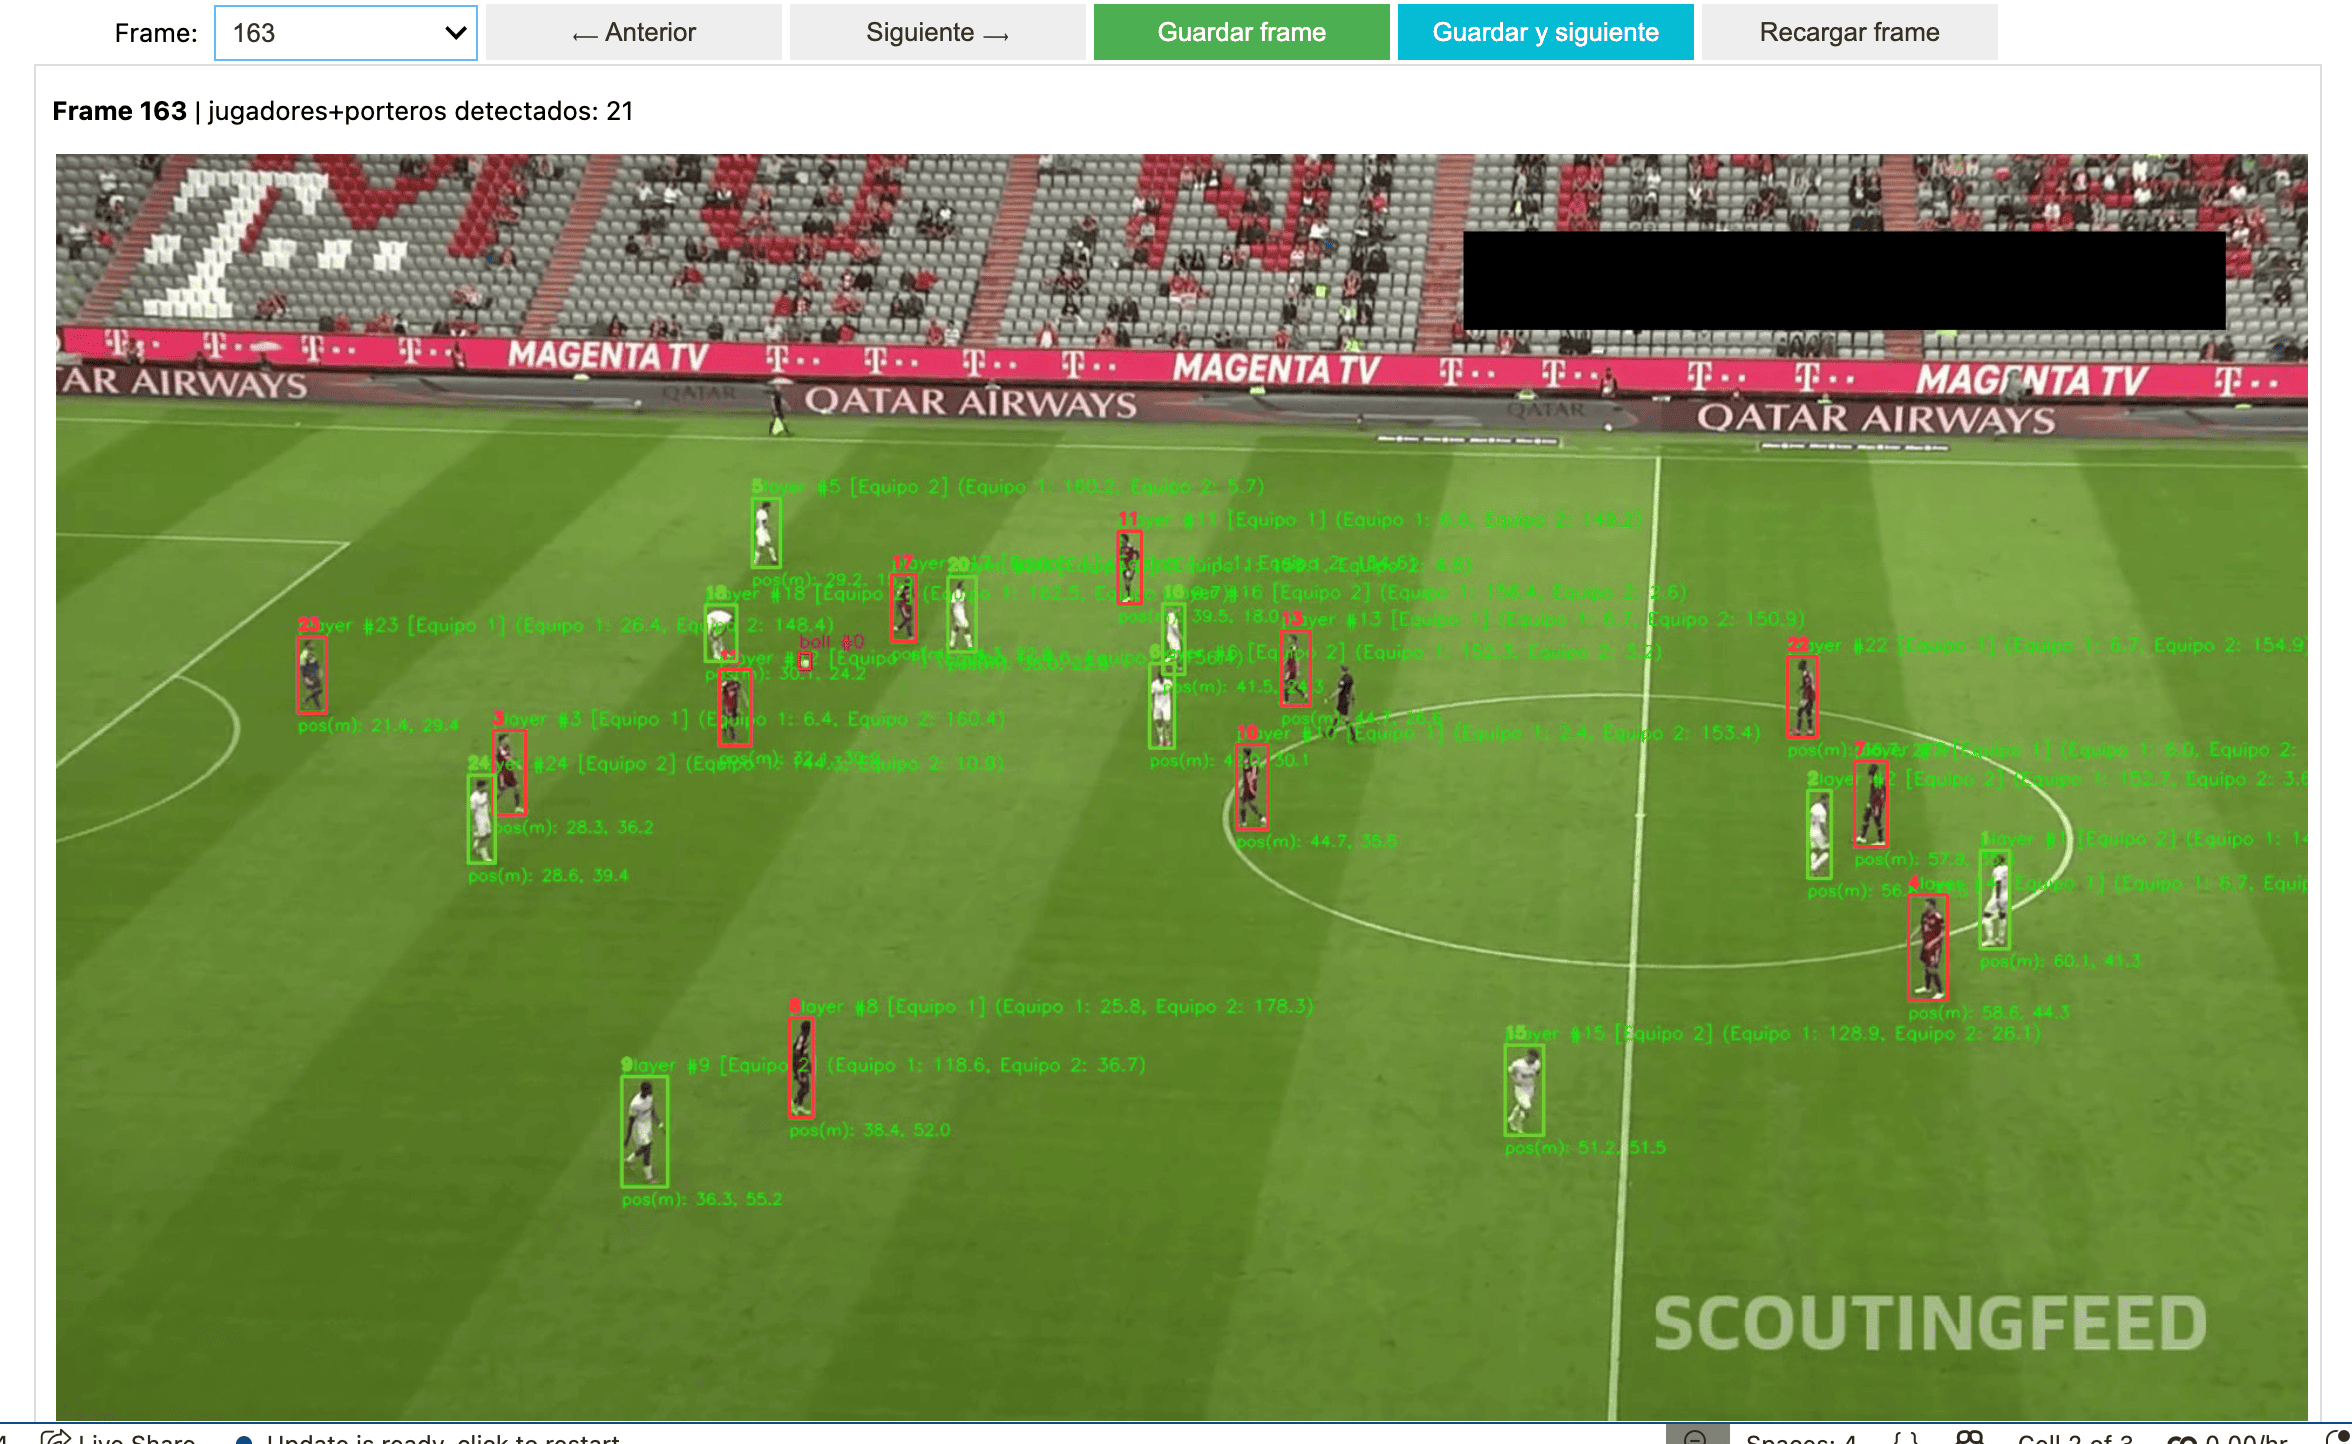
\includegraphics[width=0.49\linewidth]{Imagenes//Propias//Frame_a_etiquetar.png}
\caption[Frame de etiquetado posicional]{Frame con identificadores visibles sobre los jugadores para realizar el etiquetado posicional.}
\label{fig:frame_etiquetado_posiciones}
\end{figure}

\begin{figure}[H]
\centering
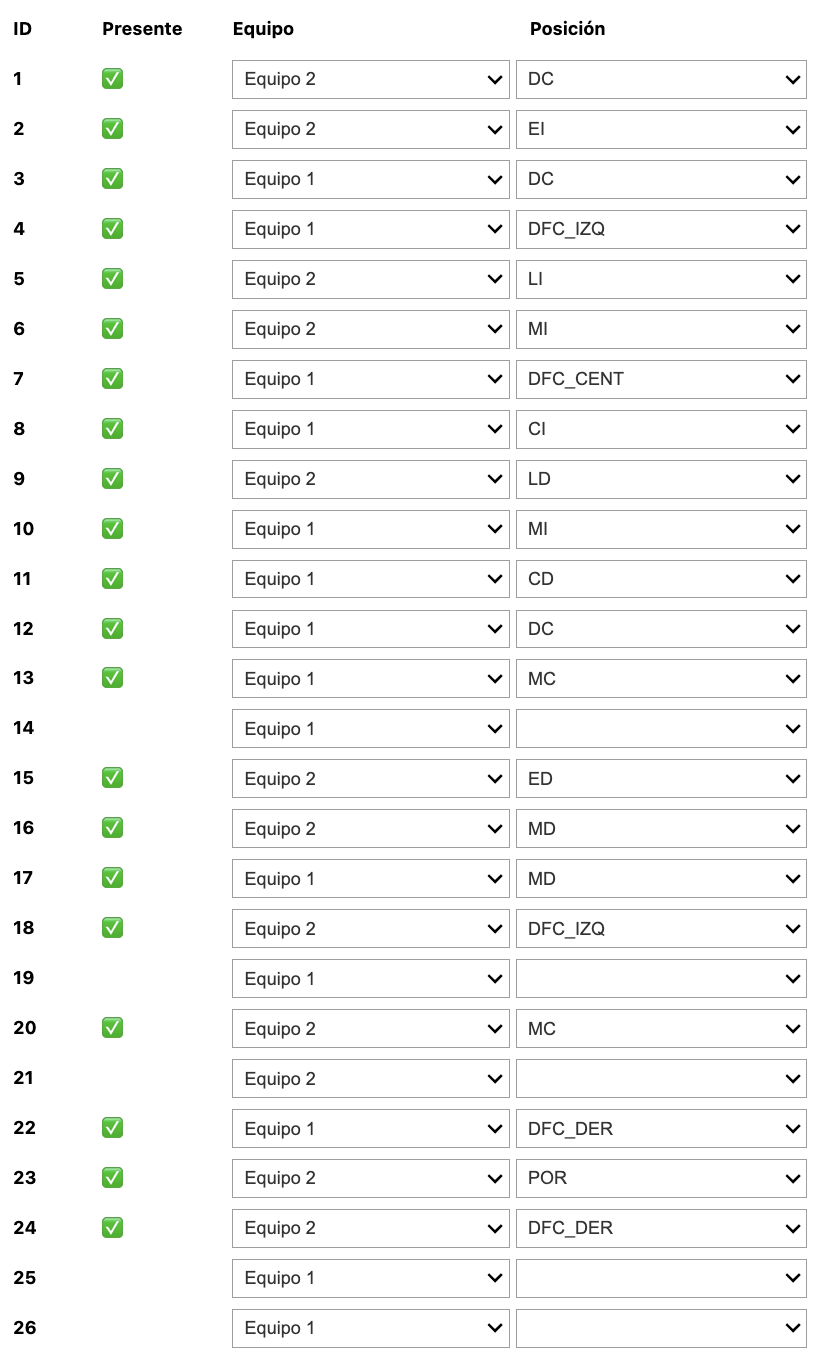
\includegraphics[width=0.49\linewidth]{Imagenes//Propias//Menu_para_etiquetar.png}
\caption[Menú de etiquetado posicional]{Menú de asignación de posición futbolística a cada identificador de tracking.}
\label{fig:menu_etiquetado_posiciones}
\end{figure}


\subsection{Normalización táctica del campo}
\label{subsec:normalizacion-tactica-campo}

Un aspecto clave es que los equipos atacan en direcciones opuestas. Sin una normalización previa, un lateral izquierdo de un equipo podría aparecer en coordenadas similares a un extremo derecho del rival. Para evitarlo, todas las muestras se transforman a una misma vista táctica antes de construir las variables de entrada del modelo.

La dirección de ataque no se introduce manualmente, sino que se infiere a partir de las observaciones del propio tracking. Cuando hay porteros detectados para ambos equipos, se toma como referencia la mediana de su coordenada normalizada \(x\): el equipo cuyo portero aparece más a la izquierda se considera asociado a la portería propia izquierda y, por tanto, se representa atacando hacia \(+x\), mientras que el otro equipo se representa atacando hacia \(-x\). Si no hay suficiente información fiable de porteros, se usa como respaldo la mediana de la coordenada \(x\) de todos los jugadores visibles del equipo.

Una vez estimada esta dirección, todas las muestras se reorientan para que ambos equipos queden expresados en el mismo sistema táctico. Si el equipo ataca hacia \(+x\), las coordenadas se mantienen. Si el equipo ataca hacia \(-x\), se aplica la transformación:

\[
x' = 1 - x, \qquad y' = 1 - y
\]

Con esta transformación, la portería propia de ambos equipos queda siempre en la misma referencia relativa, y las etiquetas izquierda/derecha conservan el mismo significado táctico independientemente del lado real del campo en el que esté jugando cada equipo.

Esta canonización es fundamental para que el modelo aprenda conceptos futbolísticos y no solo coordenadas absolutas dependientes del lado del campo. En caso contrario, dos jugadores con el mismo rol pero pertenecientes a equipos opuestos podrían ocupar regiones geométricamente parecidas en la imagen normalizada y, sin embargo, representar funciones tácticas distintas.


\subsection{Variables utilizadas}
\label{subsec:variables-inferencia-posicional}

Cada muestra del dataset representa a un jugador objetivo en un frame concreto. Para describirlo se utilizan dos bloques de información: variables propias del jugador y variables relativas a sus compañeros.

Las variables del jugador objetivo son:

\begin{itemize}
    \item \texttt{x}, \texttt{y}: coordenadas normalizadas del jugador en el campo.
    \item \texttt{dist\_left\_sideline}: distancia normalizada a la banda izquierda.
    \item \texttt{dist\_right\_sideline}: distancia normalizada a la banda derecha.
    \item \texttt{dist\_own\_goal}: distancia normalizada a la portería propia.
    \item \texttt{dist\_opponent\_goal}: distancia normalizada a la portería rival.
    \item \texttt{team\_centroid\_x}, \texttt{team\_centroid\_y}: centroide del equipo en ese frame.
    \item \texttt{dx\_centroid}, \texttt{dy\_centroid}: desplazamiento del jugador respecto al centroide del equipo.
    \item \texttt{rank\_x\_team}, \texttt{rank\_y\_team}: posición relativa del jugador dentro del equipo según los ejes del campo.
    \item \texttt{vx}, \texttt{vy}: velocidad normalizada estimada a partir del desplazamiento entre frames.
\end{itemize}

Las variables de compañeros describen el contexto espacial del jugador objetivo. Para cada compañero se incluyen:

\begin{itemize}
    \item \texttt{dx\_to\_obj}, \texttt{dy\_to\_obj}: desplazamiento relativo respecto al jugador objetivo.
    \item \texttt{dist\_to\_obj}: distancia euclídea al jugador objetivo.
    \item \texttt{x}, \texttt{y}: posición normalizada del compañero.
    \item Distancias del compañero a bandas y porterías.
    \item \texttt{vx}, \texttt{vy}: velocidad normalizada del compañero.
\end{itemize}

Se consideran como máximo 10 compañeros por muestra, ordenados por cercanía al jugador objetivo. Cuando hay menos de 10 compañeros disponibles, se rellena con ceros y se utiliza una máscara para indicar qué posiciones son reales y cuáles son padding. En el dataset final, la mediana de compañeros visibles por muestra es 9.

\subsection{Distribución de clases}

El dataset inicial presentaba un desbalanceo claro, como se muestra en la \hyperref[tab:position_class_distribution]{Tabla~\ref*{tab:position_class_distribution}}. Las clases \texttt{CI}, \texttt{CD} y \texttt{DFC\_CENT} eran las menos representadas. Tras fusionar los carrileros con los laterales, el reparto quedó más equilibrado, aunque \texttt{DFC\_CENT} siguió siendo la clase minoritaria.

\begin{table}[H]
\centering
\scriptsize
\begin{tabular}{c|c|c}
\textbf{Clase} & \textbf{Muestras antes del mapeo} & \textbf{Muestras finales} \\
\hline\hline
\texttt{CI} & 2816 & -- \\
\hline
\texttt{CD} & 2094 & -- \\
\hline
\texttt{LI} & 8013 & 10829 \\
\hline
\texttt{LD} & 7681 & 9775 \\
\hline
\texttt{DFC\_CENT} & 2897 & 2897 \\
\hline
\texttt{DFC\_IZQ} & 11896 & 11896 \\
\hline
\texttt{DFC\_DER} & 11345 & 11345 \\
\hline
\texttt{MC} & 10946 & 10946 \\
\hline
\texttt{MI} & 10562 & 10562 \\
\hline
\texttt{MD} & 11480 & 11480 \\
\hline
\texttt{EI} & 8095 & 8095 \\
\hline
\texttt{ED} & 8029 & 8029 \\
\hline
\texttt{DC} & 13665 & 13665 \\
\hline
\end{tabular}
\caption[Distribución de clases posicionales]{Distribución de clases antes y después de fusionar los carrileros \texttt{CI} y \texttt{CD} con los laterales \texttt{LI} y \texttt{LD}.}
\label{tab:position_class_distribution}
\end{table}


Una vez que se tiene el conjunto de datos etiquetado, se puede entrenar el modelo de inferencia de posiciones. Las secciones restantes de este capítulo se centran en explicar la arquitectura del modelo, su uso dentro del pipeline y en discutir los resultados obtenidos.


\subsection{Arquitectura del modelo}
\label{subsec:arquitectura-modelo-posicional}

El modelo utilizado es un Set Transformer. Como se mencionó en la \hyperref[sec:setTransformer]{Sección~\ref*{sec:setTransformer}}, esta arquitectura es adecuada porque el contexto de compañeros no es una secuencia ordenada, sino un conjunto. El orden en el que se introducen los compañeros no debería modificar la predicción. Si dos compañeros intercambian su posición en el tensor de entrada, la situación táctica sigue siendo la misma.

La entrada del modelo está formada por:

\begin{itemize}
    \item Un vector de 14 variables del jugador objetivo, descritas en la  \hyperref[subsec:variables-inferencia-posicional]{Sección~\ref*{subsec:variables-inferencia-posicional}}
    \item Un tensor de compañeros de tamaño $10 \times 11$.
    \item Una máscara binaria que indica qué compañeros existen realmente y cuáles son padding.
\end{itemize}

El modelo se divide en cuatro etapas principales, que se detallarán a continuación:

\begin{enumerate}
    \item Codificación del jugador objetivo.
    \item Codificación de cada compañero.
    \item Modelado del conjunto de compañeros mediante auto-atención.
    \item Agregación del conjunto y clasificación final.
\end{enumerate}

\subsubsection{Codificación del jugador objetivo}

El jugador objetivo se representa mediante sus 14 variables propias. Este vector se introduce en un MLP específica para el jugador objetivo, denotada como $MLP_{obj}$, que lo transforma en un embedding de dimensión fija. Este embedding resume la información individual del jugador: dónde está, a qué distancia se encuentra de bandas y porterías, cómo se sitúa respecto al centroide de su equipo y qué posición relativa ocupa dentro del bloque. Formalmente, si $x_{obj}$ es el vector de variables del jugador objetivo, se obtiene:

\[
h_{obj} = MLP_{obj}(x_{obj})
\]

donde $h_{obj}$ es el embedding individual del jugador. Esta MLP es distinta de la utilizada para codificar a los compañeros, ya que ambos tipos de entrada tienen diferente dimensionalidad y representan información distinta.

\subsubsection{Codificación de los compañeros}

Cada compañero se representa mediante 11 variables. Para codificarlos se utiliza una segunda MLP, denotada como $MLP_{comp}$, distinta de $MLP_{obj}$. Esta red se comparte entre todos los compañeros: es decir, la misma $MLP_{comp}$, con los mismos pesos aprendidos, se aplica de forma independiente a cada uno de los compañeros. De este modo, todos los compañeros se proyectan al mismo espacio latente. Formalmente, para cada compañero $i$ se calcula:

\[
h_i = MLP_{comp}(x_i)
\]

donde $x_i$ representa las variables del compañero $i$ y $h_i$ su embedding. El resultado es un conjunto de embeddings:

donde $x_i$ representa las variables del compañero $i$ y $h_i$ su embedding.

El resultado es un conjunto de embeddings:

\[
H = \{h_1, h_2, ..., h_n\}
\]

con $n \leq 10$. Si hay menos de 10 compañeros, los slots restantes se rellenan con ceros y se enmascaran.

\subsubsection{Bloques de auto-atención}

Sobre los embeddings de compañeros $H$ se aplican varios bloques de auto-atención multi-cabeza. Como se explicó en la \hyperref[sec:setTransformer]{Sección~\ref*{sec:setTransformer}}, este mecanismo permite que cada elemento del conjunto actualice su representación teniendo en cuenta al resto de elementos, sin imponer un orden secuencial sobre la entrada.

En esta implementación se utilizan bloques de auto-atención directa sobre el conjunto de compañeros, equivalentes al uso de bloques tipo SAB. No se emplean bloques ISAB, ya que el conjunto tiene un tamaño máximo de 10 compañeros y, por tanto, el coste cuadrático de la auto-atención completa no supone un problema relevante.

En cada bloque, los embeddings de los compañeros actúan simultáneamente como consultas, claves y valores:


\[
Q = HW_Q,\quad K = HW_K,\quad V = HW_V
\]

La atención se calcula como:

\[
Attention(Q,K,V)=softmax\left(\frac{QK^T}{\sqrt{d_k}}\right)V
\]

Esta operación permite aprender relaciones espaciales entre compañeros. Por ejemplo, para distinguir entre un lateral y un extremo no basta con mirar la posición del jugador objetivo; también puede ser relevante saber si tiene un compañero por delante, si forma parte de una línea defensiva, si está alineado con otros jugadores del centro del campo o si se encuentra aislado en la zona de ataque.

La atención multi-cabeza permite aprender varias relaciones espaciales en paralelo. Una cabeza puede especializarse en relaciones longitudinales, otra en relaciones laterales, otra en distancias al centroide y otra en estructuras de línea defensiva o línea ofensiva.

Tras la atención se aplica una conexión residual y una normalización:

\[
Z_1 = LayerNorm(H + Attention(H))
\]

Después se aplica una red feed-forward interna, seguida de otra normalización:

\[
Z_2 = LayerNorm(Z_1 + FFN(Z_1))
\]

La red feed-forward contiene una expansión de dimensión, activación \texttt{GELU} (Gaussian Error Linear Unit), dropout y una proyección de vuelta a la dimensión original. De esta forma, cada bloque combina relaciones entre compañeros mediante atención con transformaciones no lineales aplicadas a cada embedding.

\subsubsection{Pooling por atención}

Después de los bloques de auto-atención, el modelo dispone de un embedding contextualizado por cada compañero. Si hay \(n\) compañeros visibles, la salida de esta etapa puede escribirse como:

\[
Z \in \mathbb{R}^{n \times d}
\]

donde cada fila representa a un compañero y \(d\) es la dimensión del embedding. Sin embargo, para clasificar al jugador objetivo no se necesita una representación por compañero, sino un único vector que resuma el conjunto completo.

Para obtener este resumen se utiliza pooling por atención, basado en la idea de \textit{Pooling by Multihead Attention}, explicado también en \hyperref[sec:setTransformer]{Sección~\ref*{sec:setTransformer}}. Este mecanismo aplica la misma operación de atención descrita anteriormente, pero con una diferencia importante: las consultas no proceden de los compañeros, sino de un vector aprendible llamado \textit{seed} $S$. Este seed no representa a ningún jugador real, sino que actúa como una consulta global entrenable que aprende qué información debe extraerse del conjunto de compañeros para clasificar al jugador objetivo.

Formalmente, el pooling por atención puede escribirse como:

\[
PoolingAttention(S,Z) =
\operatorname{Attention}(SW_Q, ZW_K, ZW_V)
\]

Es decir, el seed genera la consulta \(Q\), mientras que los compañeros generan las claves \(K\) y los valores \(V\):
\[
Q = SW_Q,\quad K = ZW_K,\quad V = ZW_V
\]

donde \(S\) es el seed aprendible y \(Z\) son los embeddings de compañeros tras los bloques de auto-atención. A partir de estas matrices se calculan los pesos de atención:

\[
\alpha =
\operatorname{softmax}\left(\frac{QK^T}{\sqrt{d_k}}\right)
\]

y el resumen del conjunto se obtiene como una combinación ponderada de los valores:

\[
h_{set} = \alpha V
\]

De forma equivalente:

\[
h_{set} = PoolingAttention(S,Z)
\]


Como en este modelo se utiliza un único seed, el mecanismo produce una única salida. Por tanto, el pooling por atención reduce la dimensión asociada al número de compañeros, pasando de una representación \(n \times d\) a un único vector \(1 \times d\). Este vector resume el contexto táctico del jugador objetivo, dando más peso a los compañeros que el modelo considera más relevantes para la clasificación posicional.

\subsubsection{Clasificador final}

Finalmente, se concatena el embedding del jugador objetivo con el resumen del conjunto de compañeros:

\[
h = [h_{obj}; h_{set}]
\]

Este vector se introduce en un clasificador MLP que devuelve un logit por cada clase:

\[
logits = MLP_{cls}(h)
\]

Durante el entrenamiento se utiliza \texttt{CrossEntropyLoss}, que recibe directamente los logits. En inferencia, los logits se transforman en probabilidades mediante \texttt{softmax} y se selecciona la clase con mayor probabilidad.

\subsection{Entrenamiento}
\label{subsec:entrenamiento-modelo-posicional}

La separación del dataset se realizó por partido, no por muestras individuales. Esto es importante porque los frames consecutivos de un mismo clip son muy parecidos. Si se mezclaran frames del mismo clip entre entrenamiento y test, las métricas estarían sobreestimadas.

El split final contiene:

\begin{itemize}
    \item 82122 muestras de entrenamiento.
    \item 13603 muestras de validación.
    \item 13794 muestras de test.
\end{itemize}

Como se comenta en la sección anterior, el modelo produce, para cada muestra, un vector de logits \(z \in \mathbb{R}^{C}\), donde \(C\) es el número de clases posicionales. Estos logits se transforman en probabilidades mediante la función \textit{softmax}:

\[
p_c =
\frac{\exp(z_c)}
{\sum_{j=1}^{C} \exp(z_j)}
\]

donde \(p_c\) representa la probabilidad asignada a la clase \(c\).

Durante el entrenamiento se utilizó \texttt{CrossEntropyLoss}. Para una etiqueta real \(y\), la pérdida de entropía cruzada mide el desacuerdo entre la distribución objetivo y la distribución predicha por el modelo. En el caso básico, con etiquetas \textit{one-hot}, se expresa como:

\[
\mathcal{L} = - \log(p_y)
\]

donde \(p_y\) es la probabilidad predicha para la clase correcta.

Como el dataset presenta cierto desbalanceo entre clases, se utilizaron pesos de clase en la función de pérdida. Estos pesos se calcularon de forma inversamente proporcional a la frecuencia de cada clase en el conjunto de entrenamiento:

\[
w_c = \frac{N}{C \cdot n_c}
\]

donde \(N\) es el número total de muestras de entrenamiento, \(C\) es el número de clases y \(n_c\) es el número de muestras de la clase \(c\). De esta forma, los errores cometidos sobre clases poco representadas tienen mayor peso en la pérdida que los errores sobre clases frecuentes. La pérdida ponderada puede escribirse como:

\[
\mathcal{L} = - w_y \log(p_y)
\]

donde \(w_y\) es el peso asociado a la clase correcta.

Además, en el modelo final se aplicó \textit{label smoothing}. En lugar de entrenar con una etiqueta completamente concentrada en la clase correcta, se suaviza ligeramente la distribución objetivo. Para una muestra de clase real \(y\), la etiqueta suavizada se define como:

\[
\tilde{y}_c =
\begin{cases}
1 - \varepsilon + \frac{\varepsilon}{C}, & \text{si } c = y \\
\frac{\varepsilon}{C}, & \text{si } c \neq y
\end{cases}
\]

donde \(\varepsilon\) es el factor de suavizado. Con esta modificación, la pérdida pasa a calcularse sobre todas las clases:

\[
\mathcal{L} =
- \sum_{c=1}^{C} w_c \, \tilde{y}_c \log(p_c)
\]

El objetivo de esta técnica es evitar que el modelo se vuelva excesivamente confiado en sus predicciones. Esto resulta especialmente útil en esta tarea, ya que algunas posiciones futbolísticas son ambiguas desde el punto de vista espacial. Por ejemplo, un lateral, un interior y un extremo pueden ocupar zonas similares dependiendo de la fase de juego.

La métrica principal utilizada para seleccionar el mejor modelo fue el \textit{macro-F1}:
\[
MacroF1 =
\frac{1}{C}
\sum_{c=1}^{C} F1_c
\]

Esta métrica da el mismo peso a todas las clases, independientemente de su frecuencia. Por ello es más adecuada que la accuracy en un problema con clases desbalanceadas, ya que permite evaluar si el modelo funciona razonablemente bien también sobre las posiciones menos representadas.


\subsection{Grid search de hiperparámetros}
\label{subsec:grid-search-posicional}

Para optimizar el modelo se realizaron varios barridos de hiperparámetros. La \hyperref[tab:rejilla_grid_posiciones_base]{Tabla~\ref*{tab:rejilla_grid_posiciones_base}} resume la rejilla base utilizada en las Pruebas 1 y 3, mientras que la \hyperref[tab:rejilla_grid_posiciones_refine]{Tabla~\ref*{tab:rejilla_grid_posiciones_refine}} resume la rejilla de refinamiento usada en la Prueba 4. Cada prueba se evaluó con métricas agregadas y con su matriz de confusión en test, como se detalla a continuación.

\begin{table}[H]
\centering
\scriptsize
\resizebox{\textwidth}{!}{%
\begin{tabular}{c|c}
\textbf{Hiperparámetro} & \textbf{Valores explorados} \\
\hline\hline
Perfiles de anchura &
\((64,128,128,128),\ (128,256,192,256),\ (128,256,256,256),\ (256,384,256,384)\) \\
\hline
\texttt{objective\_num\_layers} & \(\{1,2\}\) \\
\hline
\texttt{ff\_expansion} & \(\{2,4\}\) \\
\hline
\texttt{num\_set\_blocks} & \(\{3,4,5\}\) \\
\hline
\texttt{learning\_rate} & \(\{10^{-3},\ 5\cdot10^{-4}\}\) \\
\hline
Regularización \((\texttt{dropout},\ \texttt{weight\_decay})\) &
\((0{.}10,\ 10^{-4});\ (0{.}15,\ 10^{-4});\ (0{.}20,\ 5\cdot10^{-4});\ (0{.}25,\ 5\cdot10^{-4});\ (0{.}30,\ 10^{-3})\) \\
\hline
Fijos & \(\texttt{batch\_size}=512,\ \texttt{num\_heads}=4,\ \texttt{epochs}=40\) \\
\hline
Núm. total de runs & \(480\) \\
\hline
\end{tabular}%
}
\caption[Rejilla base de las búsquedas de hiperparámetros]{Rejilla base utilizada en los barridos principales (Pruebas 1 y 3). Cada perfil de anchura se expresa como \((\texttt{teammate\_embed\_dim},\texttt{objective\_hidden\_dim},\texttt{set\_hidden\_dim},\texttt{fusion\_hidden\_dim})\), que corresponden respectivamente a la dimensión del embedding de compañeros, la dimensión oculta del codificador del jugador objetivo, la dimensión interna de los bloques de atención sobre el set y la dimensión de la capa de fusión previa al clasificador.}
\label{tab:rejilla_grid_posiciones_base}
\end{table}

\begin{table}[H]
\centering
\scriptsize
\resizebox{\textwidth}{!}{%
\begin{tabular}{c|c}
\textbf{Hiperparámetro} & \textbf{Valores explorados} \\
\hline\hline
Familias base & top-\(3\) de la Prueba 3 \\
\hline
\texttt{learning\_rate} & \(\{3\cdot10^{-4},\ 2\cdot10^{-4},\ 10^{-4}\}\) \\
\hline
\texttt{label\_smoothing} & \(\{0{.}05,\ 0{.}10\}\) \\
\hline
\texttt{weight\_decay} & \(\{7{.}5\cdot10^{-4},\ 1{.}5\cdot10^{-3},\ 2\cdot10^{-3}\}\) \\
\hline
\texttt{dropout} & \(\{0{.}18,\ 0{.}22,\ 0{.}27,\ 0{.}33,\ 0{.}35\}\) \\
\hline
Fijos & \(\texttt{batch\_size}=512,\ \texttt{num\_heads}=4,\ \texttt{epochs}=40\) \\
\hline
Núm. total de runs & \(108\) \\
\hline
\end{tabular}%
}
\caption[Rejilla de refinamiento de hiperparámetros]{Rejilla de refinamiento usada en la Prueba 4}
\label{tab:rejilla_grid_posiciones_refine}
\end{table}

\subsubsection{Prueba 1: grid search con 13 clases}
La primera búsqueda mantuvo la taxonomía inicial, con \texttt{CI} y \texttt{CD} como clases independientes. Se ejecutaron 480 combinaciones variando anchura de los embeddings y capas ocultas del modelo, profundidad del codificador del jugador objetivo, el número de bloques de atención, el factor de expansión de la capa de feed-forward y la regularización y optimización (\textit{dropout}, \textit{learning\_rate}, \textit{weight\_decay}). La mejor configuración alcanzó un \textit{macro-F1} de 0.3096 en validación y 0.4022 en test, tal y como muestra la \hyperref[tab:grid_13_metrics]{Tabla~\ref*{tab:grid_13_metrics}}

\begin{table}[H]
\centering
\scriptsize
\begin{tabular}{c|c|c|c}
\textbf{Conjunto} & \textbf{Accuracy} & \textbf{Macro-F1} & \textbf{Weighted-F1} \\
\hline\hline
Validación & 0.3779 & 0.3096 & 0.3684 \\
\hline
Test & 0.4223 & 0.4022 & 0.4158 \\
\hline
\end{tabular}
\caption{Métricas de la mejor configuración del grid search con 13 clases.}
\label{tab:grid_13_metrics}
\end{table}

En resumen, los mejores resultados de validación tendieron a concentrarse en configuraciones con regularización moderada-baja (\texttt{dropout}=0.10, \texttt{weight\_decay}=1e-4) y \texttt{learning\_rate}=5e-4. Por otro lado, la variación de anchura y profundidad del modelo no mostró un patrón dominante claro en esta prueba, lo que sugiere que, con 13 clases, el rendimiento estuvo más condicionado por la regularización que por incrementos de capacidad.

La matriz de confusión de la \hyperref[fig:confusion_grid_13]{Figura~\ref*{fig:confusion_grid_13}} muestra que \texttt{CI} y \texttt{CD} eran clases inestables. En muchos casos se confundían con laterales, extremos o interiores. Esta observación motivó la fusión de carrileros con laterales.


\begin{figure}[H]
\centering
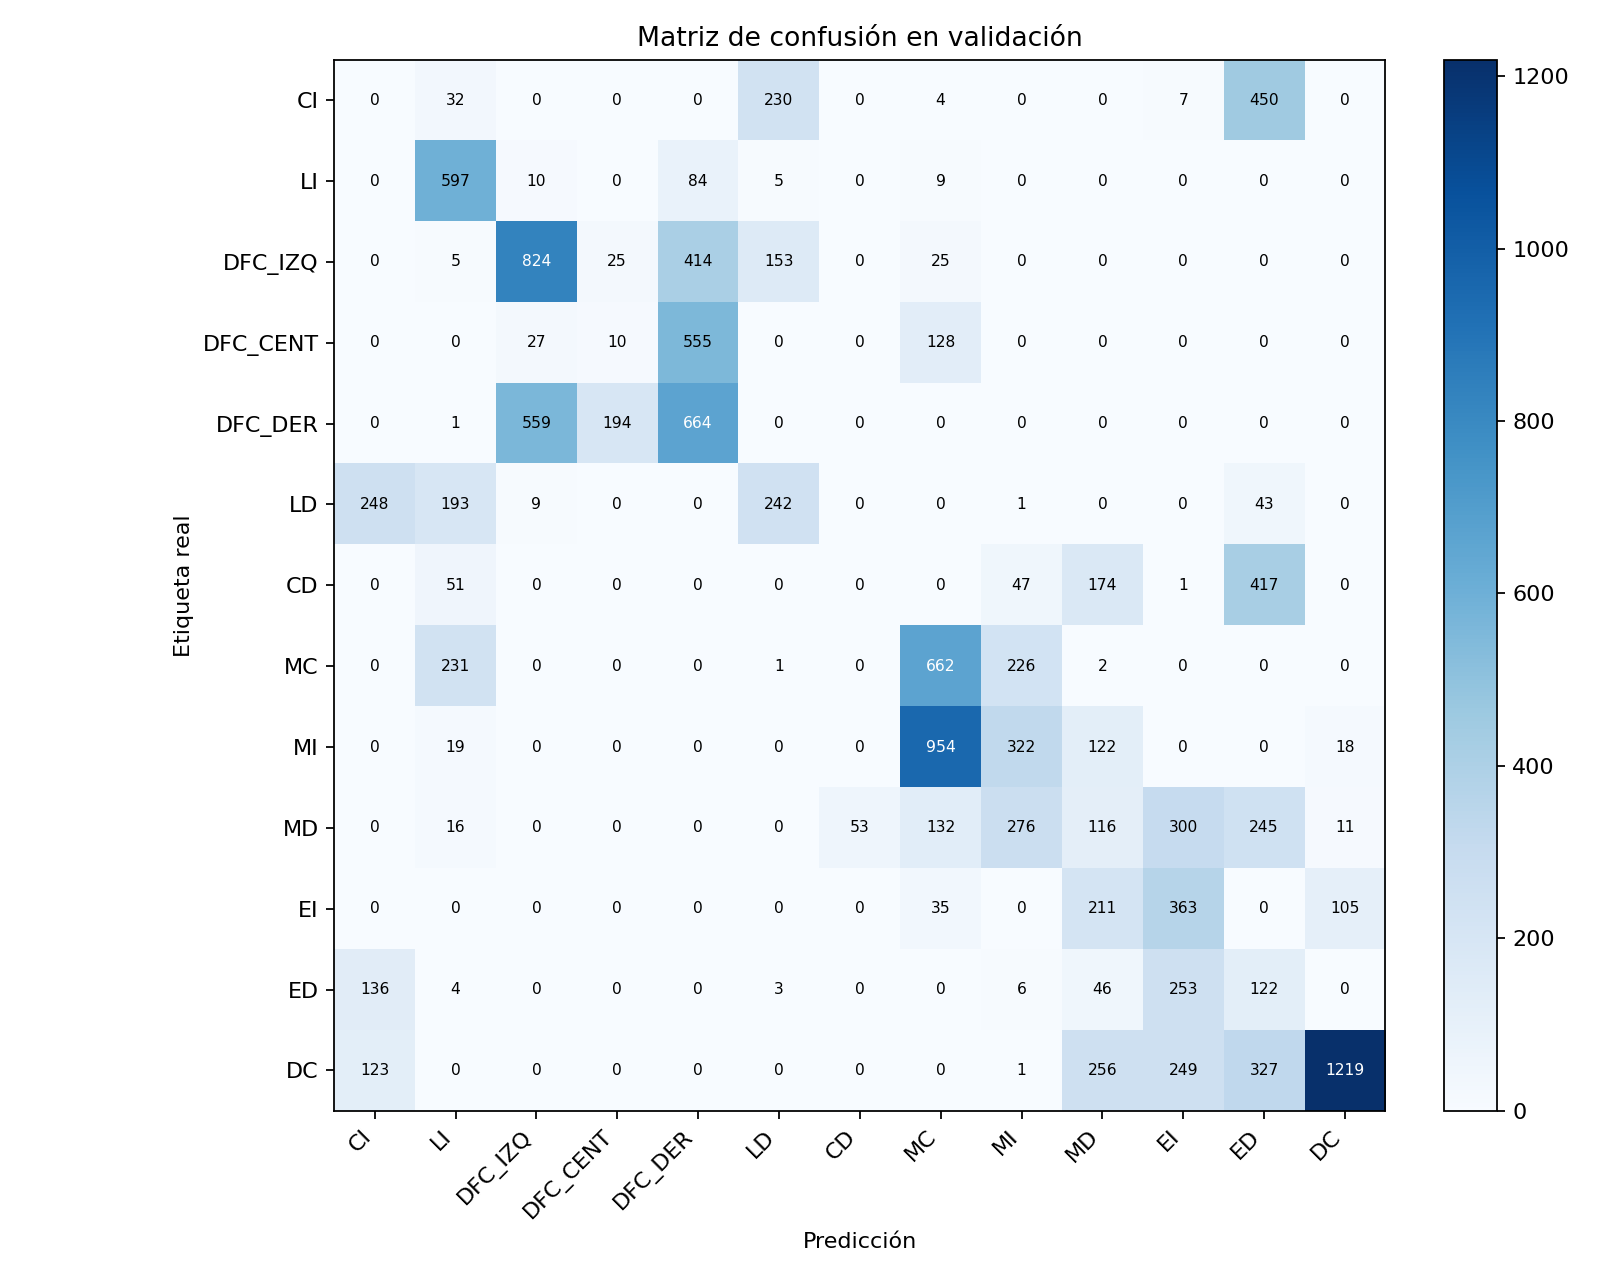
\includegraphics[width=0.8\linewidth]{Imagenes//Propias//matriz_confusion_grid_13.png}
\caption{Matriz de confusión en test del mejor modelo entrenado con 13 clases.}
\label{fig:confusion_grid_13}
\end{figure}


\subsubsection{Prueba 2: fusión de carrileros con laterales}

En la segunda prueba se mantuvo la mejor configuración de la Prueba 1 y se aplicó el mapeo:

\[
\texttt{CI} \rightarrow \texttt{LI},\quad \texttt{CD} \rightarrow \texttt{LD}
\]

El número de clases pasó de 13 a 11. Se puede observar en la \hyperref[tab:grid_merged_metrics]{Tabla~\ref*{tab:grid_merged_metrics}} y en la \hyperref[fig:confusion_merged]{Figura~\ref*{fig:confusion_merged}} que el rendimiento aumentó de forma clara, especialmente en validación (\(+0.2169\) en \textit{macro-F1}) y también en test (\(+0.0823\) en \textit{macro-F1}) respecto a la Prueba 1.

Esta prueba confirmó que, con el volumen de datos disponible, separar carrileros y laterales introducía más ruido que información útil.

\begin{table}[H]
\centering
\scriptsize
\begin{tabular}{c|c|c|c}
\textbf{Conjunto} & \textbf{Accuracy} & \textbf{Macro-F1} & \textbf{Weighted-F1} \\
\hline\hline
Validación & 0.5563 & 0.5265 & 0.5628 \\
\hline
Test & 0.5240 & 0.4845 & 0.5156 \\
\hline
\end{tabular}
\caption{Métricas tras fusionar carrileros con laterales.}
\label{tab:grid_merged_metrics}
\end{table}

\begin{figure}[H]
\centering
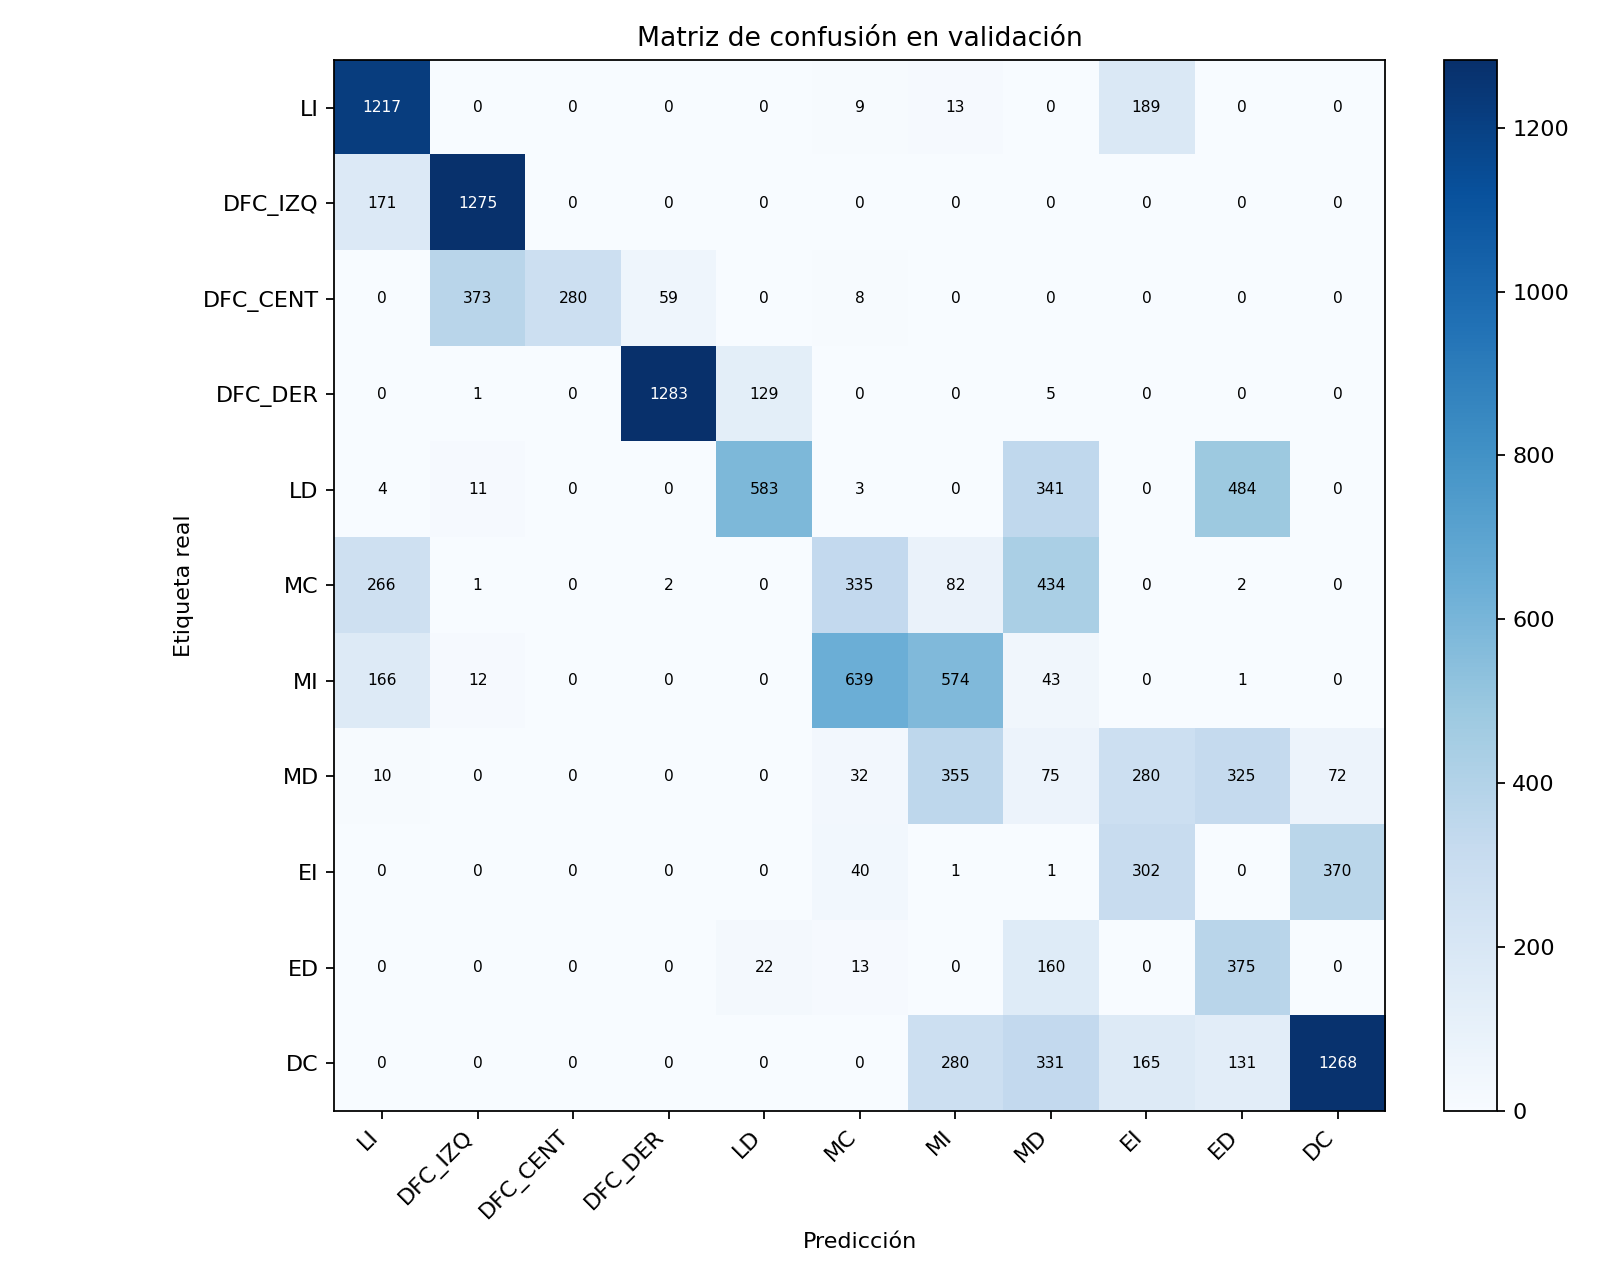
\includegraphics[width=0.8\linewidth]{Imagenes//Propias//matriz_confusion_carrileros_fusionados.png}
\caption{Matriz de confusión en test tras fusionar \texttt{CI} con \texttt{LI} y \texttt{CD} con \texttt{LD}.}
\label{fig:confusion_merged}
\end{figure}


\subsubsection{Prueba 3: grid search completo con 11 clases}

Tras comprobar que el mapeo era beneficioso, se repitió un grid search completo con 11 clases. Se exploraron de nuevo 480 combinaciones. La mejor configuración utilizó una arquitectura más compacta, 5 bloques de atención y mayor regularización.

La \hyperref[tab:grid_11_metrics]{Tabla~\ref*{tab:grid_11_metrics}} y la \hyperref[fig:confusion_grid_11]{Figura~\ref*{fig:confusion_grid_11}} resumen los resultados obtenidos. Aunque la validación mejoró claramente frente a la Prueba 2 (\(+0.0666\) en \textit{macro-F1}), el rendimiento en test apenas aumentó (\(+0.0048\) en \textit{macro-F1}). Esto sugiere que algunas configuraciones empezaban a adaptarse demasiado al clip de validación.

\begin{table}[H]
\centering
\scriptsize
\begin{tabular}{c|c|c|c}
\textbf{Conjunto} & \textbf{Accuracy} & \textbf{Macro-F1} & \textbf{Weighted-F1} \\
\hline\hline
Validación & 0.6168 & 0.5931 & 0.6207 \\
\hline
Test & 0.5170 & 0.4893 & 0.5096 \\
\hline
\end{tabular}
\caption{Métricas del grid search completo con 11 clases.}
\label{tab:grid_11_metrics}
\end{table}

\begin{figure}[H]
\centering
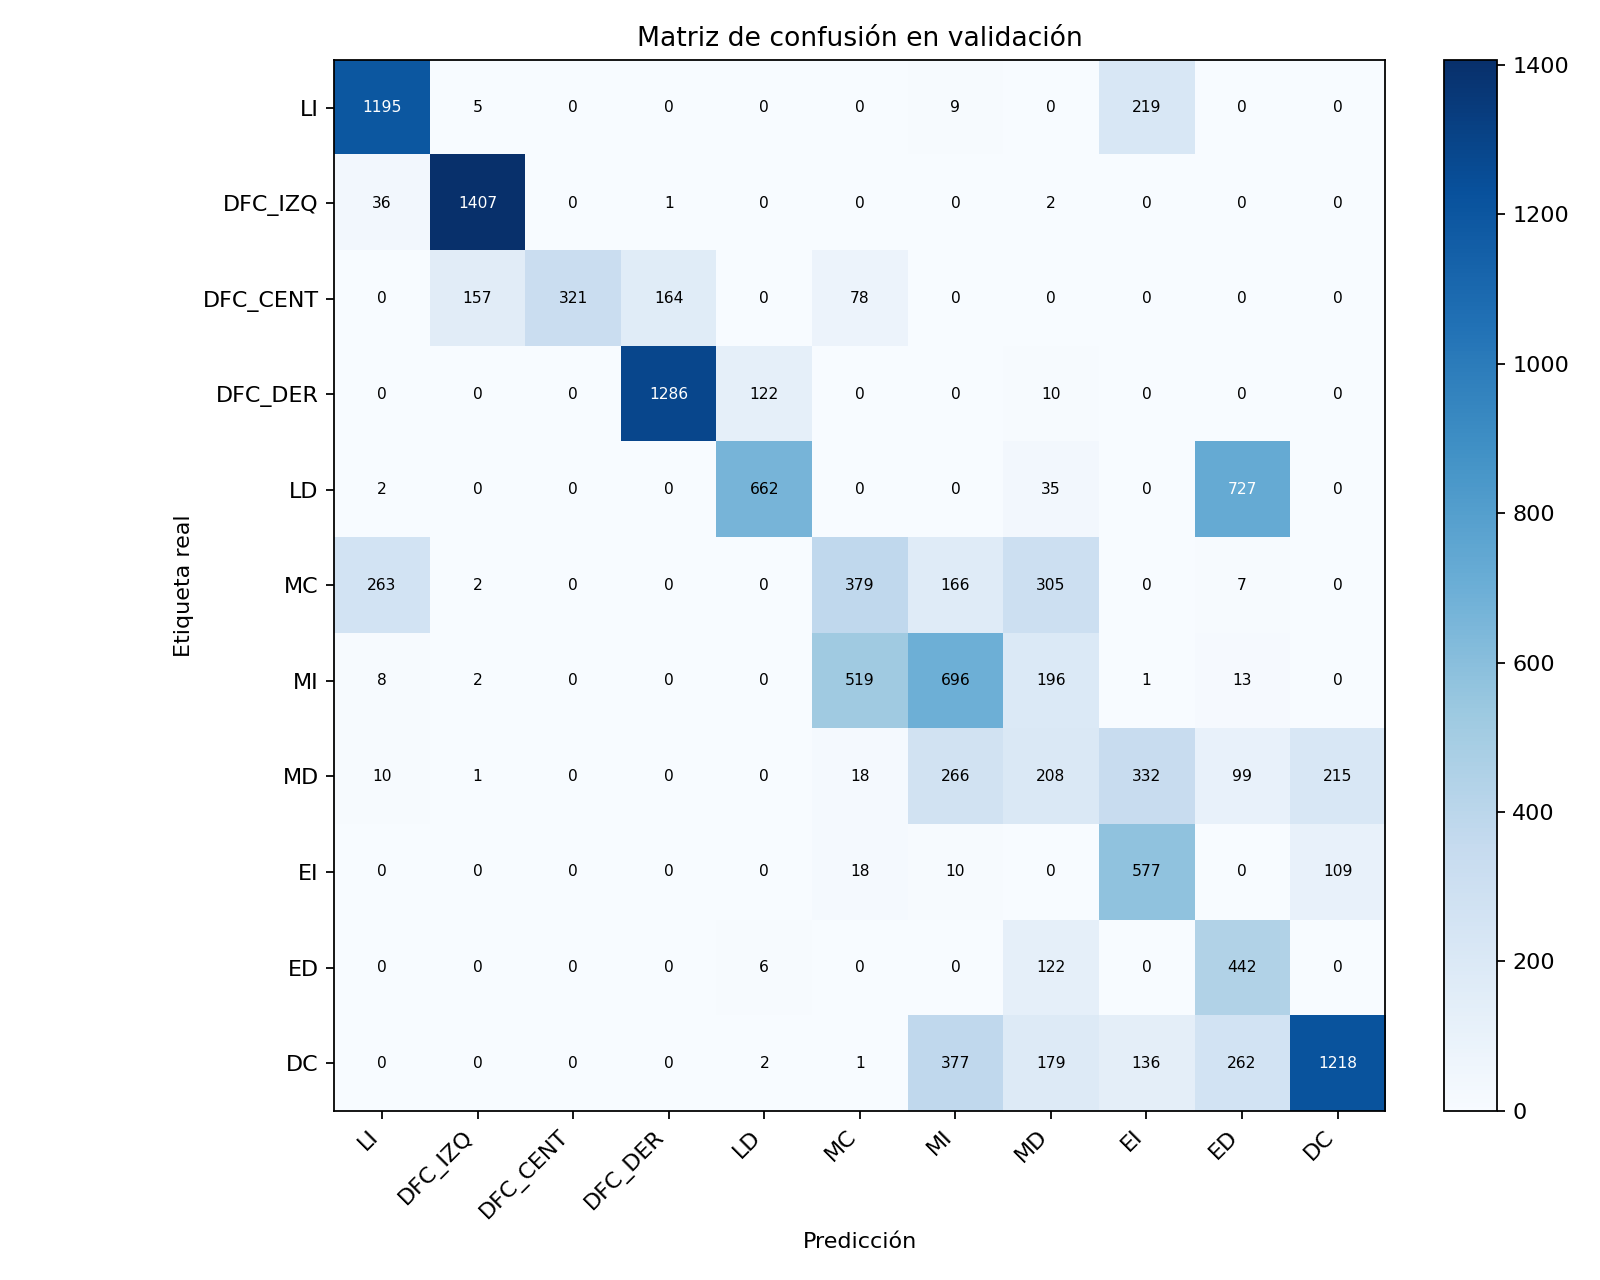
\includegraphics[width=0.8\linewidth]{Imagenes//Propias//matriz_confusion_grid_11.png}
\caption[Matriz de confusión del mejor modelo del grid search]{Matriz de confusión en test del mejor modelo del grid search completo con 11 clases.}
\label{fig:confusion_grid_11}
\end{figure}


\subsubsection{Prueba 4: refinamiento de los tres mejores modelos}

En la última fase se tomaron los tres mejores modelos del grid anterior y se refinó alrededor de ellos. En lugar de volver a cruzar todos los parámetros, se mantuvieron fijas tres familias arquitectónicas base y se probaron nuevos valores de \texttt{learning\_rate}, \texttt{weight\_decay}, \texttt{dropout} y \texttt{label\_smoothing}. Las tres arquitecturas base utilizadas se resumen en la \hyperref[tab:arquitecturas_refinamiento_posiciones]{Tabla~\ref*{tab:arquitecturas_refinamiento_posiciones}}.

\begin{table}[H]
\centering
\scriptsize
\begin{tabular}{c|c|c|c|c}
\textbf{Modelo} & \textbf{Perfil de anchura} & \texttt{objective\_num\_layers} & \texttt{ff\_expansion} & \texttt{num\_set\_blocks} \\
\hline\hline
1 & \((64,128,128,128)\) & \(2\) & \(4\) & \(5\) \\
\hline
2 & \((128,256,256,256)\) & \(1\) & \(2\) & \(5\) \\
\hline
3 & \((128,256,256,256)\) & \(1\) & \(2\) & \(3\) \\
\hline
\end{tabular}
\caption[Arquitecturas base del refinamiento]{Arquitecturas base utilizadas en la fase de refinamiento de hiperparámetros. El perfil de anchura se expresa como \((\texttt{teammate\_embed\_dim},\texttt{objective\_hidden\_dim},\texttt{set\_hidden\_dim},\texttt{fusion\_hidden\_dim})\).}
\label{tab:arquitecturas_refinamiento_posiciones}
\end{table}

En total se ejecutaron 108 entrenamientos.

El mejor modelo final obtuvo un \textit{macro-F1} de 0.6068 en validación y 0.5588 en test, como se muestra en la \hyperref[tab:modelo_final_metricas]{Tabla~\ref*{tab:modelo_final_metricas}}. La matriz de confusión en test se representa en la \hyperref[fig:confusion_modelo_final]{Figura~\ref*{fig:confusion_modelo_final}}.

\begin{table}[H]
\centering
\scriptsize
\begin{tabular}{c|c|c|c}
\textbf{Conjunto} & \textbf{Accuracy} & \textbf{Macro-F1} & \textbf{Weighted-F1} \\
\hline\hline
Validación & 0.6333 & 0.6068 & 0.6358 \\
\hline
Test & 0.5804 & 0.5588 & 0.5703 \\
\hline
\end{tabular}
\caption{Métricas del modelo final tras el refinamiento de hiperparámetros.}
\label{tab:modelo_final_metricas}
\end{table}

\begin{figure}[H]
\centering
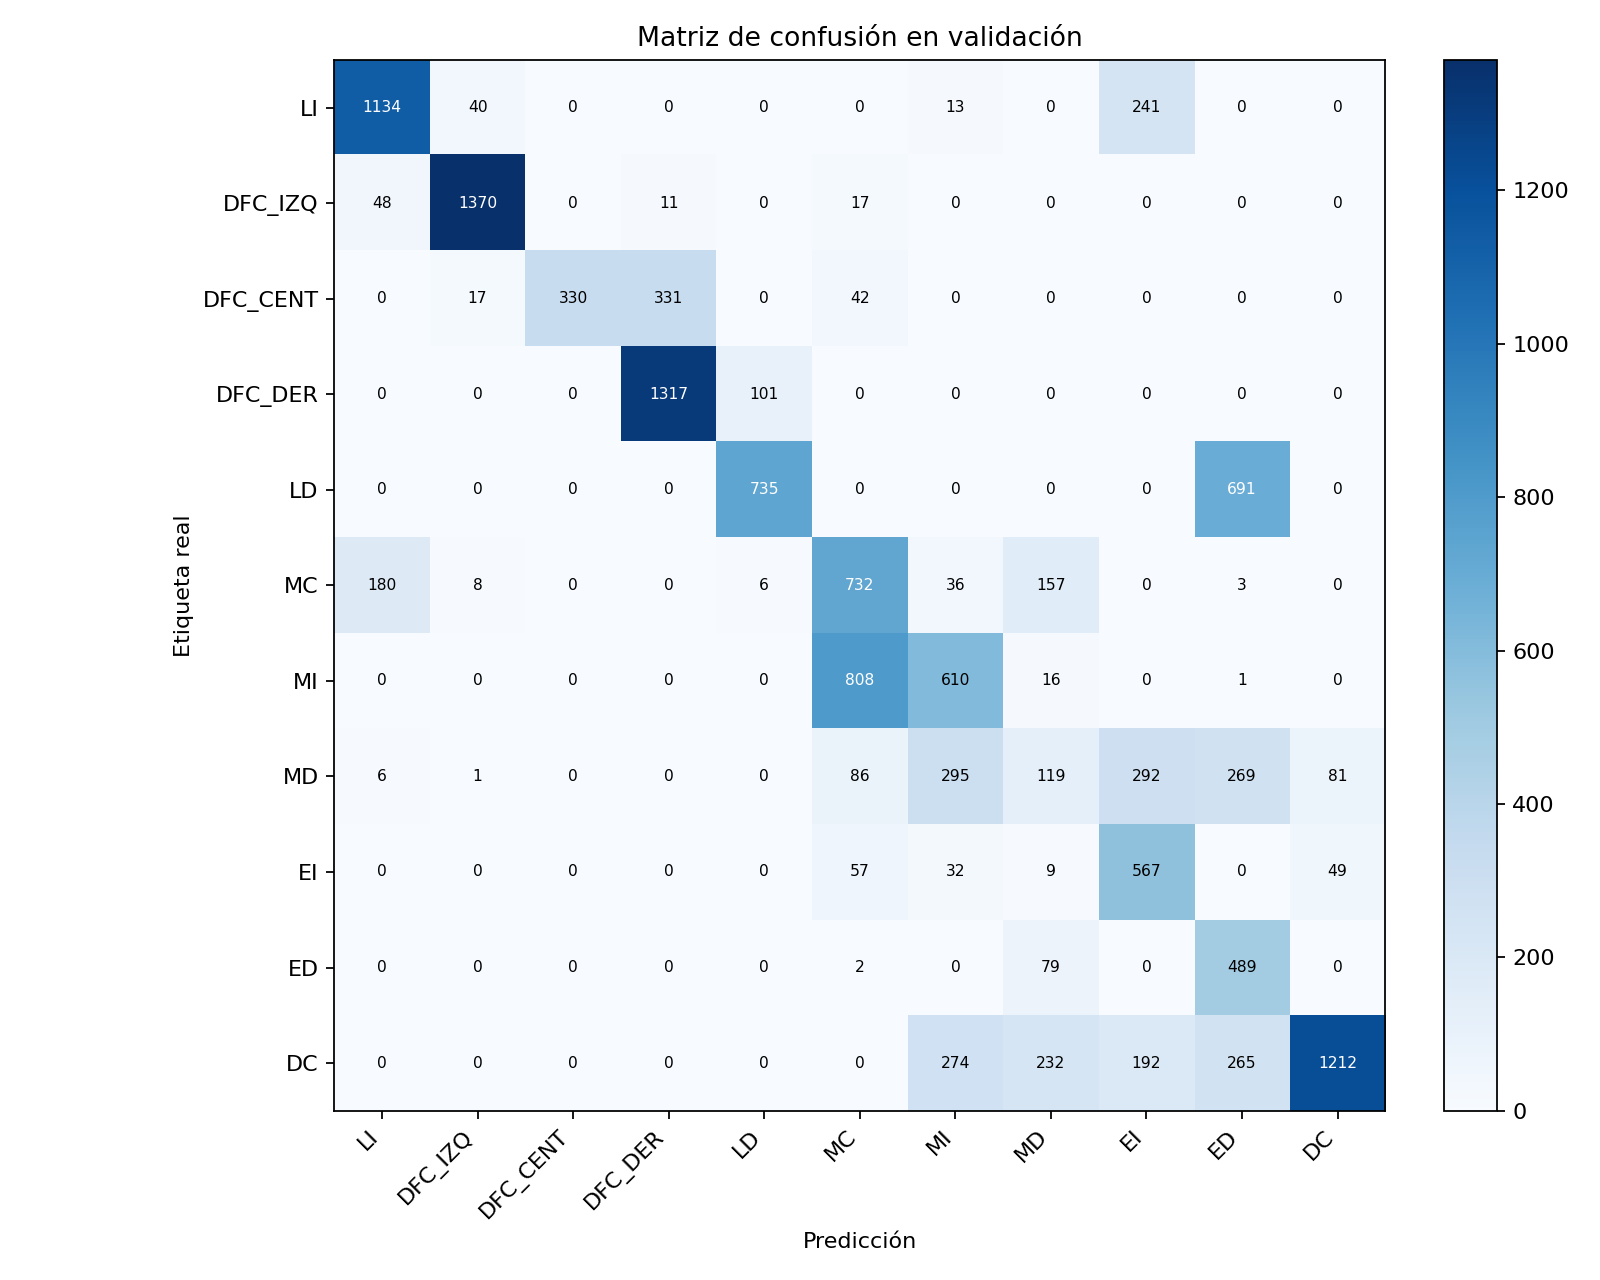
\includegraphics[width=0.8\linewidth]{Imagenes//Propias//matriz_confusion_modelo_final.png}
\caption{Matriz de confusión en test del modelo final.}
\label{fig:confusion_modelo_final}
\end{figure}

La curva de entrenamiento de la \hyperref[fig:curvas_entrenamiento_modelo_final]{Figura~\ref*{fig:curvas_entrenamiento_modelo_final}} muestra que el mejor punto se alcanza en las primeras épocas. A partir de ese momento, el rendimiento en entrenamiento sigue mejorando, pero la validación deja de mejorar de forma consistente. Este comportamiento indica sobreajuste temprano, algo esperable por la fuerte correlación entre frames de un mismo clip y por el tamaño limitado del conjunto de partidos etiquetados. Por ello se utiliza parada temprana y se selecciona el checkpoint con mayor \textit{macro-F1} de validación.

\begin{figure}[H]
\centering
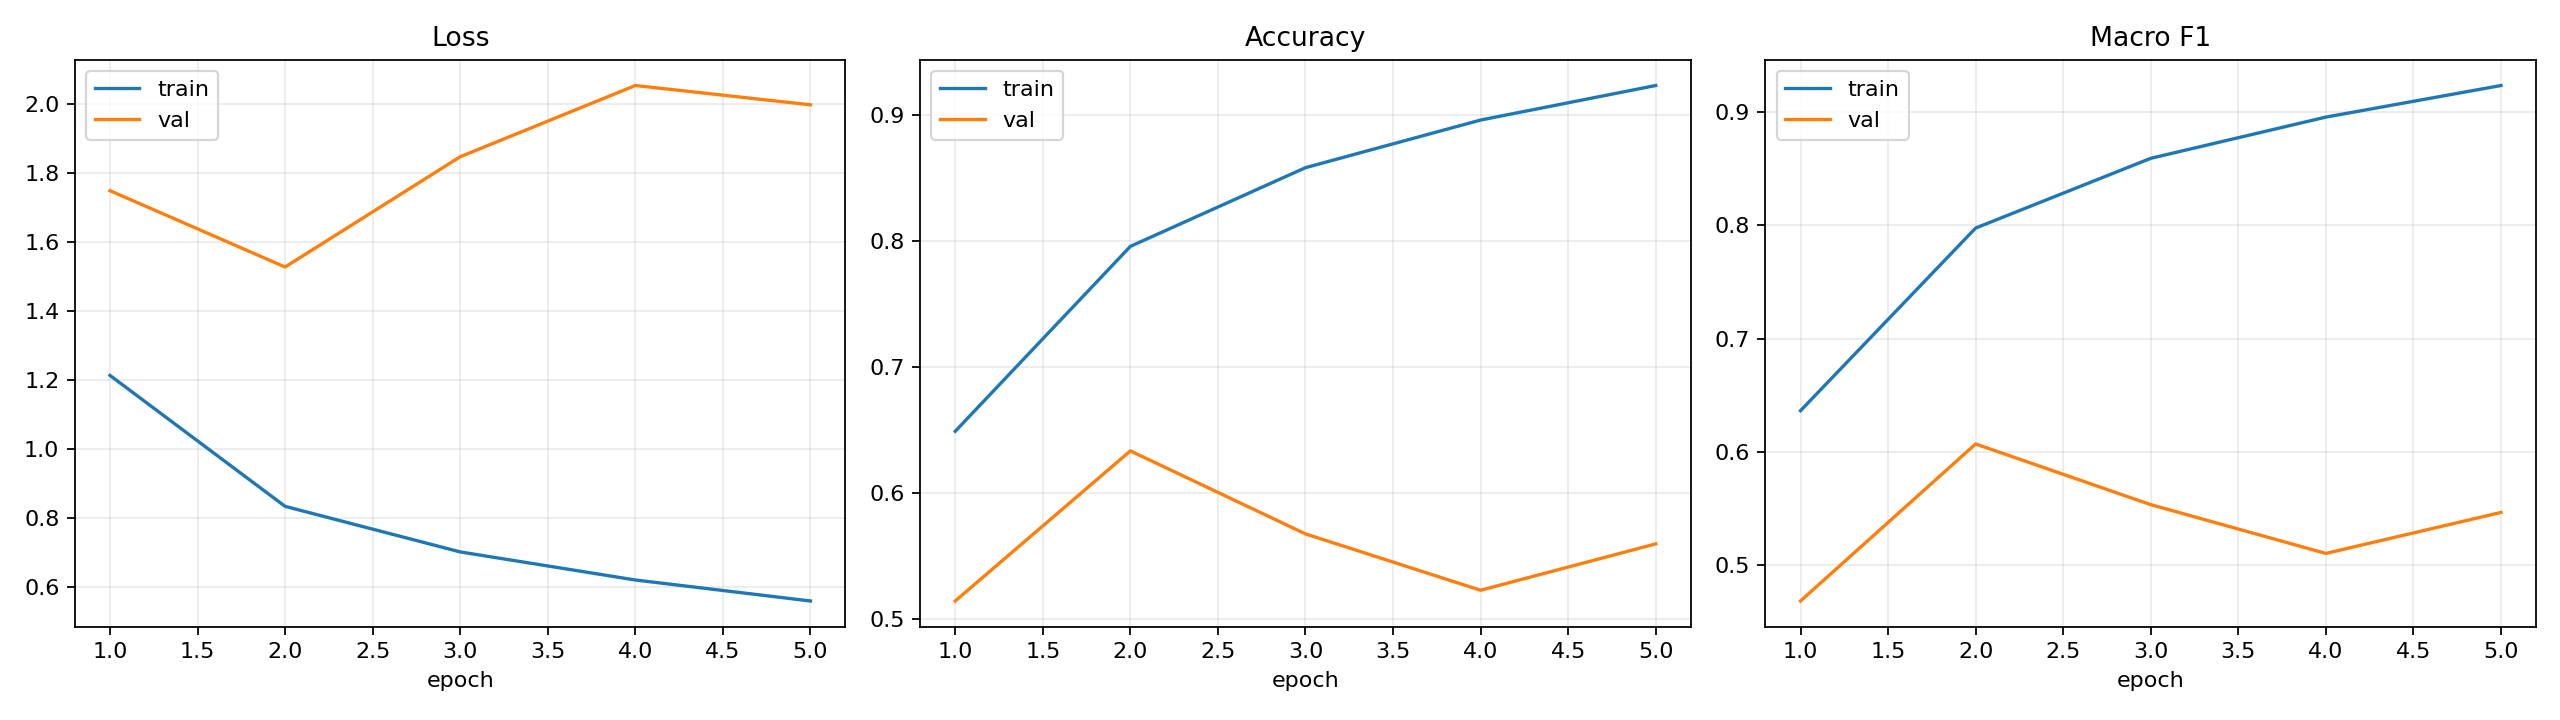
\includegraphics[width=0.49\linewidth]{Imagenes//Propias//curvas_entrenamiento_modelo_final.png}
\caption[Curvas entrenamiento del modelo final]{Evolución de la pérdida, accuracy y macro-F1 durante el entrenamiento del modelo final.}
\label{fig:curvas_entrenamiento_modelo_final}
\end{figure}


\subsection{Hiperparámetros del modelo final}
\label{subsec:hiperparametros-modelo-posicional}

El modelo final utiliza la siguiente configuración especificada en la \hyperref[tab:hiperparametros_modelo_final]{Tabla~\ref*{tab:hiperparametros_modelo_final}}:

\begin{table}[H]
\centering
\scriptsize
\begin{tabular}{c|c}
\textbf{Parámetro} & \textbf{Valor} \\
\hline\hline
\texttt{teammate\_embed\_dim} & 128 \\
\hline
\texttt{objective\_hidden\_dim} & 256 \\
\hline
\texttt{set\_hidden\_dim} & 256 \\
\hline
\texttt{fusion\_hidden\_dim} & 256 \\
\hline
\texttt{objective\_num\_layers} & 1 \\
\hline
\texttt{num\_set\_blocks} & 5 \\
\hline
\texttt{num\_heads} & 4 \\
\hline
\texttt{ff\_expansion} & 2 \\
\hline
\texttt{dropout} & 0.27 \\
\hline
\texttt{label\_smoothing} & 0.05 \\
\hline
\texttt{learning\_rate} & 0.0002 \\
\hline
\texttt{weight\_decay} & 0.0015 \\
\hline
\texttt{batch\_size} & 512 \\
\hline
\end{tabular}
\caption{Hiperparámetros del modelo final.}
\label{tab:hiperparametros_modelo_final}
\end{table}

El parámetro \texttt{teammate\_embed\_dim} controla la anchura de la MLP que codifica cada compañero antes de introducirlo en la atención. El parámetro \texttt{objective\_hidden\_dim} define la dimensión oculta usada para representar al jugador objetivo.

Por otro lado, \texttt{set\_hidden\_dim} es la dimensión interna del Set Transformer. Es uno de los valores más importantes, ya que determina la capacidad del modelo para representar relaciones entre compañeros. \texttt{fusion\_hidden\_dim} define la anchura del clasificador final tras concatenar el embedding del jugador objetivo y el resumen del conjunto.

El parámetro \texttt{objective\_num\_layers} indica cuántas capas ocultas tiene la MLP del jugador objetivo. En el modelo final se usa una única capa, lo que sugiere que las variables individuales son suficientemente expresivas y que añadir más profundidad aumentaba el riesgo de sobreajuste.

El número de bloques de auto-atención que se aplican sobre los compañeros está definido por \texttt{num\_set\_blocks}. El modelo final usa 5 bloques, permitiendo refinar varias veces las relaciones espaciales del conjunto. \texttt{num\_heads} indica el número de cabezas de atención en paralelo. Con 4 cabezas, el modelo puede aprender distintos tipos de relaciones tácticas simultáneamente.

Para controlar cuánto se expande la dimensión interna dentro del bloque \textit{feed-forward} de cada bloque de atención se utiliza \texttt{ff\_expansion}. \texttt{dropout} introduce regularización apagando aleatoriamente neuronas durante el entrenamiento. El valor final, 0.27, es relativamente alto, coherente con el sobreajuste observado.

Con \texttt{label\_smoothing} se suavizan las etiquetas durante el entrenamiento. En vez de asignar probabilidad 1 a la clase correcta y 0 al resto, reparte una pequeña fracción de probabilidad entre las demás clases. Esto es útil porque algunas posiciones son tácticamente ambiguas.

Por último, \texttt{learning\_rate} controla el tamaño de los pasos del optimizador, y \texttt{weight\_decay} penaliza pesos demasiado grandes. Ambos contribuyen a estabilizar el entrenamiento y mejorar la generalización.

\subsection{Resultados por clase}
\label{subsec:resultados-clase-posicional}

El modelo final alcanza una accuracy de 0.5804 y un \textit{macro-F1} de 0.5588 en test. En la \hyperref[tab:set_transformer_test_by_class]{Tabla~\ref*{tab:set_transformer_test_by_class}} se puede observar que las mejores clases son \texttt{DFC\_IZQ}, \texttt{ED}, \texttt{DFC\_DER}, \texttt{DC} y \texttt{LI}. Las clases más difíciles son \texttt{DFC\_CENT}, \texttt{MD}, \texttt{MC} y \texttt{MI}.

\begin{table}[H]
\centering
\scriptsize
\begin{tabular}{c|c|c|c|c}
\textbf{Clase} & \textbf{Precisión test} & \textbf{Recall test} & \textbf{F1 test} & \textbf{Soporte test} \\
\hline\hline
\texttt{LI} & 0.6078 & 0.5985 & 0.6031 & 1432 \\
\hline
\texttt{DFC\_IZQ} & 0.9026 & 0.8560 & 0.8787 & 1451 \\
\hline
\texttt{DFC\_CENT} & 0.6272 & 0.1434 & 0.2335 & 739 \\
\hline
\texttt{DFC\_DER} & 0.5910 & 0.6723 & 0.6290 & 1367 \\
\hline
\texttt{LD} & 0.5820 & 0.5363 & 0.5582 & 1337 \\
\hline
\texttt{MC} & 0.4194 & 0.4783 & 0.4469 & 1403 \\
\hline
\texttt{MI} & 0.4724 & 0.4823 & 0.4773 & 1188 \\
\hline
\texttt{MD} & 0.4848 & 0.3457 & 0.4036 & 1478 \\
\hline
\texttt{EI} & 0.4263 & 0.9294 & 0.5845 & 694 \\
\hline
\texttt{ED} & 0.5464 & 0.9874 & 0.7035 & 715 \\
\hline
\texttt{DC} & 0.7674 & 0.5322 & 0.6285 & 1990 \\
\hline
\end{tabular}
\caption{Resultados por clase del modelo final sobre el conjunto de test.}
\label{tab:set_transformer_test_by_class}
\end{table}

Estos resultados son coherentes con la naturaleza de la tarea. Las posiciones de banda y algunos defensas tienen patrones espaciales más estables, mientras que los mediocentros e interiores dependen más de la fase de juego, de intercambios posicionales y del contexto colectivo.

\subsection{Reentrenamiento con \textit{train+val}}
\label{subsec:reentrenamiento-train-val-posicional}

Una vez seleccionado el mejor modelo mediante el \textit{grid search}, se realizó una prueba adicional para comprobar si el rendimiento podía mejorar utilizando más datos durante el entrenamiento. La idea consistía en unir los conjuntos de entrenamiento y validación, entrenar de nuevo el modelo con los hiperparámetros previamente seleccionados y evaluar el resultado únicamente sobre el conjunto de test. Esta prueba tiene sentido porque el modelo mostraba síntomas de sobreajuste temprano, por lo que cabía pensar que disponer de más muestras durante el entrenamiento podría mejorar su capacidad de generalización.

En esta prueba se entrenó el modelo durante 2 épocas, que era la época óptima obtenida en el proceso de validación anterior. El conjunto \textit{train+val} contenía 95725 muestras, mientras que el conjunto de test se mantuvo separado y no se utilizó para tomar decisiones durante el entrenamiento.

Como se observa en la \hyperref[tab:comparacion_train_val_posiciones]{Tabla~\ref*{tab:comparacion_train_val_posiciones}}, el reentrenamiento con \textit{train+val} no mejoró los resultados en test. Aunque el modelo alcanzó sobre \textit{train+val} una \textit{accuracy} de 0.8890 y un \textit{macro-F1} de 0.8924, su rendimiento sobre test fue inferior al del modelo seleccionado mediante validación. Esto indica que añadir la partición de validación al entrenamiento no redujo el sobreajuste, sino que probablemente aumentó la adaptación del modelo a los fragmentos ya vistos. En este caso, todos los vídeos etiquetados proceden del mismo partido, por lo que la caída no se debe a un cambio completo de dominio entre partidos distintos. Por este motivo, se decidió mantener como modelo principal el seleccionado mediante validación, ya que ofrecía una mejor generalización sobre el fragmento reservado como test.

\begin{table}[H]
    \centering
    \scriptsize
    \begin{tabular}{p{0.36\linewidth}|c|c|c}
        \textbf{Modelo} & \textbf{Acc. test} & \textbf{Macro-F1 test} & \textbf{Weighted-F1 test} \\
        \hline\hline
        Modelo seleccionado por validación & 0.5804 & 0.5588 & 0.5703 \\
        \hline
        Reentrenado con \textit{train+val} & 0.5161 & 0.4833 & 0.5020 \\
        \hline
    \end{tabular}
    \caption[Comparación de estrategias de entrenamiento]{Comparación entre el modelo seleccionado en validación y el modelo reentrenado con \textit{train+val}.}
    \label{tab:comparacion_train_val_posiciones}
\end{table}


\subsection{Asignación táctica final de posiciones}
\label{subsec:asignacion-tactica-final-posiciones}

Tras obtener las probabilidades del Set Transformer, la inferencia no termina escogiendo simplemente la clase con mayor probabilidad para cada jugador. Esa predicción directa existe, pero se utiliza únicamente como una primera estimación. Posteriormente se aplica una fase de asignación táctica cuyo objetivo es que las posiciones finales sean coherentes con la alineación esperada de cada equipo.

Para ello, el flujo combina dos niveles de asignación: una asignación inmediata por frame y una reasignación estable por segmentos temporales de identidad.

\subsubsection{Asignación online por frame}

En cada frame, el modelo recibe como entrada los tracks activos generados en las fases previas del pipeline. Para cada track correspondiente a un jugador de campo, se construye una muestra formada por dos bloques de información: por un lado, las 14 variables propias del jugador, descritas en la \hyperref[subsec:variables-inferencia-posicional]{Sección~\ref*{subsec:variables-inferencia-posicional}}, y por otro, una matriz de contexto de tamaño \(10 \times 11\), que representa hasta 10 compañeros del mismo equipo mediante 11 variables por compañero.

Una vez construida esta representación $x_i$, la muestra se introduce en el Set Transformer descrito en las secciones anteriores. El modelo devuelve, para cada track, un vector de logits asociado a las clases posicionales aprendidas. Estos logits se transforman posteriormente en probabilidades mediante la función \textit{softmax}, obteniendo así una estimación de pertenencia del jugador a cada una de las posiciones posibles. La predicción de rol de cada jugador se obtiene mediante la clase con mayor probabilidad:

\[
\hat{y}_i = \arg\max_{c \in \mathcal{C}} p_i(c)
\]

Sin embargo, esta predicción no constituye todavía la posición final de cada jugador. El Set Transformer proporciona una estimación probabilística inicial para cada una de las 11 clases aprendidas (\texttt{LI}, \texttt{DFC\_IZQ}, \texttt{DFC\_CENT}, \texttt{DFC\_DER}, \texttt{LD}, \texttt{MC}, \texttt{MI}, \texttt{MD}, \texttt{EI}, \texttt{ED}, \texttt{DC}), pero después se aplica una fase de asignación táctica cuyo objetivo es que las posiciones finales sean coherentes con la alineación esperada de cada equipo. Este paso evita configuraciones tácticamente imposibles; por ejemplo, que varios jugadores queden asignados simultáneamente como delanteros mientras otras plazas defensivas del once esperado quedan vacías.

Para realizar esta corrección se construye una matriz de costes entre los tracks activos y las plazas tácticas esperadas en la alineación. Cada fila de la matriz representa un track detectado en el frame y cada columna representa una plaza del once esperado. Por ejemplo, si una formación contiene dos delanteros, existirán dos columnas distintas asociadas a la clase \texttt{DC}.

El coste entre el track \(i\) y la plaza táctica \(j\) se calcula a partir de la probabilidad que el modelo asigna a la clase correspondiente para dicho track y penalizaciones relacionadas con la familia espacial y la posición en el campo. De forma simplificada, puede expresarse como:

\[
C_{ij}=\min_{\ell\in A(s_j)}
\left[
-\log\left(p_i(\ell)+\varepsilon\right)
+\mathrm{pen}_{\mathrm{compat}}(s_j,\ell)
+\mathrm{pen}_{\mathrm{geo}}(i,s_j)
\right]
\]


donde \(s_j\) es la clase posicional asociada a la plaza \(j\), \(A(s_j)\) es el conjunto de etiquetas del modelo compatibles con esa plaza \(s_j\), \(\ell\) es una etiqueta candidata dentro del conjunto \(A(s_j)\), \(p_i(\ell)\) es la probabilidad asignada por el modelo al track \(i\) para la etiqueta \(\ell\), y \(\varepsilon\) es un valor pequeño para evitar el logaritmo de cero. De este modo, una probabilidad alta produce un coste bajo, mientras que una probabilidad baja produce un coste alto.

En esta implementación solo se relaja la compatibilidad en las posiciones de banda. 
Para ello se definen dos familias laterales:
\[
\mathcal{B}_{\mathrm{izq}}=\{\texttt{LI},\texttt{MI},\texttt{EI}\},
\qquad
\mathcal{B}_{\mathrm{der}}=\{\texttt{LD},\texttt{MD},\texttt{ED}\}.
\]

El conjunto de etiquetas compatibles con una plaza \(s\) se define como:
\[
A(s)=
\begin{cases}
\mathcal{B}_{\mathrm{izq}}, & \text{si } s\in \mathcal{B}_{\mathrm{izq}},\\[0.3em]
\mathcal{B}_{\mathrm{der}}, & \text{si } s\in \mathcal{B}_{\mathrm{der}},\\[0.3em]
\{s\}, & \text{en otro caso}.
\end{cases}
\]

La penalización de compatibilidad entre plaza y etiqueta se define como:
\[
\mathrm{pen}_{\mathrm{compat}}(s,\ell)=
\begin{cases}
0 & s=\ell,\\
0 & \text{si } \mathrm{fam}(s)=\varnothing \ \text{o}\ \mathrm{fam}(\ell)=\varnothing,\\
1000 & \text{si } \mathrm{fam}(s)\neq \mathrm{fam}(\ell),\\
0.35 & \text{si } \mathrm{fam}(s)=\mathrm{fam}(\ell)\ \text{y falta alguna ancla},\\
\lambda_{\mathrm{compat}}\, d_{\mathrm{anch}}(a_s,a_\ell) & \text{si } \mathrm{fam}(s)=\mathrm{fam}(\ell)\ \text{con anclas disponibles},
\end{cases}
\]
donde \(\mathrm{fam}(\cdot)\in\{\texttt{LEFT},\texttt{RIGHT},\varnothing\}\) denota la familia lateral del rol
(\(\varnothing\) para roles sin familia lateral), y en esta implementación \(\lambda_{\mathrm{compat}}=1.10\).

La penalización geométrica se define como:
\[
\mathrm{pen}_{\mathrm{geo}}(i,s)=\lambda_{\mathrm{geo}}\; d_{\mathrm{anch}}\big((x_i,y_i),a_s\big),
\]
donde \((x_i,y_i)\) es la posición normalizada del track \(i\), \(a_s\) es el ancla táctica de la plaza \(s\), y \(\lambda_{\mathrm{geo}}\) es el peso geométrico.
donde \((x_i,y_i)\) es la posición normalizada del track \(i\), \(a_s\) es el ancla táctica de la plaza \(s\), y \(\lambda_{\mathrm{geo}}\) es el peso geométrico (en esta implementación, \(\lambda_{\mathrm{geo}}=1.35\)). Este parámetro controla cuánto influye la coherencia espacial en el coste total: valores más altos penalizan con mayor intensidad los emparejamientos alejados de su ancla táctica, mientras que valores más bajos priorizan en mayor medida la probabilidad del modelo.

La distancia ponderada a ancla utilizada en ambos términos es:
\[
d_{\mathrm{anch}}(u,v)=\sqrt{(u_x-v_x)^2+\left(\alpha_y\,(u_y-v_y)\right)^2},
\]
con \(\alpha_y\) como factor de ponderación vertical (en esta implementación, \(\alpha_y=1.20\)), de modo que diferencias en el eje \(y\), es decir sobr el eje del ancho del campo, se penalizan ligeramente más que diferencias equivalentes en \(x\).

Una vez construida la matriz de costes \(C\), se aplica el algoritmo húngaro para obtener la asignación global $\sigma^*$ de menor coste entre tracks y plazas tácticas:

\[
\sigma^* =
\arg\min_{\sigma}
\sum_i C_{i,\sigma(i)}
\]

donde \(\sigma(i)\) indica la plaza asignada al track \(i\). El algoritmo debe cumplir además que una misma plaza táctica no pueda ser asignada a dos tracks distintos. Esta optimización no toma decisiones de forma independiente para cada jugador, sino que busca una solución conjunta para todo el equipo. Por ejemplo, aunque varios tracks tengan alta probabilidad de pertenecer a la clase \texttt{DC}, el algoritmo solo podrá asignarlos a plazas de delantero si esas plazas existen realmente en el once esperado. El resultado final es una asignación de roles coherente con la alineación introducida.


\subsubsection{Apertura y cierre de segmentos}
\label{subsec:aperturaSegmentos}

La estabilidad temporal se organiza mediante segmentos de identidad. Esta decisión está motivada por el objetivo final de la inferencia posicional: no se busca únicamente estimar la posición táctica de un jugador en un frame concreto, sino utilizar esa posición para asociar el track con el futbolista real de la alineación. Dado que se dispone del once inicial, si se infiere de forma estable que un jugador ocupa una determinada plaza táctica, es posible asociarlo con el nombre correspondiente en la alineación introducida.

Idealmente, un track representaría una única identidad durante toda su vida. En ese caso, bastaría con inferir su posición una vez, o acumular evidencia a lo largo del track completo, para asignarle un jugador real. Sin embargo, en la práctica el tracking puede sufrir pérdidas, reasociaciones o cambios de identidad. Por tanto, no se puede asumir que un mismo \textit{track id} corresponda siempre al mismo futbolista durante todo el vídeo.

Por este motivo, en lugar de tratar cada track como una identidad indivisible, su vida temporal se divide en segmentos. Un segmento representa un tramo continuo del track en el que el sistema considera razonable acumular evidencia para una misma identidad táctica. Mientras no aparezcan señales fuertes de ruptura, las nuevas asignaciones se siguen incorporando al segmento activo.

La apertura de un nuevo segmento se activa en dos tipos de situaciones. La primera corresponde a casos en los que el ByteTrack no conservó la identidad temporal, y fue posteriormente la capa canónica de tracking, quién reasoció esa identidad. La segunda aparece cuando se detecta un salto posicional grande acompañado también de un cambio de rol respecto al rol dominante acumulado en el segmento. En estos casos, el segmento anterior se cierra, se almacena su estado agregado y se abre un nuevo segmento vacío para empezar a acumular evidencia desde ese punto.

De esta forma, un track no define necesariamente una única identidad final. En su lugar, son sus segmentos los que actúan como unidades temporales de identidad. Cada segmento acumula su propia evidencia posicional y puede asociarse posteriormente con una plaza táctica de la alineación. Este mecanismo evita mezclar en una misma memoria temporal observaciones que podrían pertenecer a futbolistas distintos o a tramos del track cuya continuidad no es completamente fiable.

\subsubsection{Acumulación de evidencia por segmento}

Una vez definido el segmento activo de cada track, el sistema acumula sobre él las asignaciones obtenidas frame a frame tras aplicar la corrección táctica mediante el algoritmo húngaro. Por tanto, la identidad táctica de un segmento no se decide a partir de una única predicción aislada, sino a partir del conjunto de evidencias recogidas durante su duración.

Para cada segmento activo se almacenan distintas estadísticas: el número de observaciones, los conteos de votos por rol, la suma de confianzas asociadas a cada rol, el rol dominante en el histórico del segmento, el rol dominante en una ventana temporal reciente y estadísticas espaciales resumidas del jugador.

Además de los votos categóricos, el sistema conserva información sobre la posición media del jugador en el campo, sus posiciones recientes y la última posición válida observada para poder determinar la continuidad o cierre del segmento, como se explica en la sección anterior.

\subsubsection{Reasignación estable por segmentos}

Una vez acumulada evidencia sobre los segmentos activos, se aplica un segundo nivel de asignación táctica. A diferencia de la asignación online por frame, esta reasignación no trabaja con predicciones instantáneas de tracks, sino con segmentos temporales que resumen la evidencia recogida durante varios frames.

Para cada equipo se construye una nueva matriz de costes entre los segmentos activos y las plazas tácticas del once esperado. Cada fila representa un segmento y cada columna una plaza de la alineación. El coste entre un segmento \(i\) y una plaza táctica \(j\) combina tres fuentes de información: la frecuencia con la que el segmento ha sido asignado al rol asociado a esa plaza, la confianza acumulada en dichas asignaciones y la coherencia geométrica entre la posición media del segmento y el ancla táctica de la plaza.

De forma simplificada, este coste puede expresarse como:

\[
C^{seg}_{ij}
=
\left(1-\frac{n_i(s_j)}{N_i}\right)
-
\lambda_{conf}\,\bar{q}_i(s_j)
+
\lambda_{geo}\,d(\mu_i,a_j)
\]

donde \(s_j\) es el el rol de la plaza \(j\), \(n_i(s_j)\) es el número de votos del segmento \(i\) para ese \textit{slot}, \(N_i\) es el total de observaciones del segmento, \(\bar{q}_i(s_j)\) es la confianza media acumulada de esos votos, \(\mu_i\) es la posición media del segmento y \(a_j\) el ancla táctica de la plaza.

Sobre esta matriz se aplica de nuevo el algoritmo húngaro, obteniendo una asignación global de segmentos a plazas tácticas. Esta asignación se interpreta como el rol estable del segmento, ya que no depende de una única predicción del modelo, sino del conjunto de votos acumulados durante la vida del segmento.

En algunas alineaciones, además, existen plazas duplicadas que el modelo base no distingue como clases separadas. Por ejemplo, el modelo predice \texttt{DC} como clase única, pero el once esperado puede requerir dos plazas diferenciadas (\texttt{DC\_IZQ} y \texttt{DC\_DCHO}), De forma análoga puede ocurrir con \texttt{MC}. Para resolver esta desambiguación lateral, cada segmento mantiene un histórico de su relación espacial con ambas bandas (distancia acumulada a banda izquierda y a banda derecha). Cuando dos segmentos compiten por una pareja duplicada de una misma clase base, ese histórico lateral se utiliza para decidir cuál ocupa la plaza izquierda y cuál la derecha, obteniendo una asignación final más estable y tácticamente interpretable.

\subsubsection{Salida final y trazabilidad}

La salida final conserva información de los distintos niveles de inferencia. Por un lado, se mantiene la predicción instantánea del modelo para el frame actual; por otro, la asignación corregida por el algoritmo húngaro a nivel de frame; y, finalmente, la asignación estable obtenida tras acumular evidencia en el segmento.
